\documentclass[a4paper, 11pt]{article}
\usepackage[margin=3cm]{geometry}
\usepackage[]{fontenc}
\usepackage[utf8]{inputenc}
\usepackage[italian]{babel}
\usepackage{geometry}
\geometry{a4paper, top=2cm, bottom=3cm, left=1.5cm, right=1.5cm, heightrounded, bindingoffset=5mm}
\usepackage{amsmath}
\usepackage{amssymb}
\usepackage{gensymb}
\usepackage{graphicx}
\usepackage{psfrag,amsmath,amsfonts,verbatim}
\usepackage{xcolor}
\usepackage{color,soul}
\usepackage{fancyhdr}
\usepackage{indentfirst}
\usepackage{graphicx}
\usepackage{newlfont}
\usepackage{amssymb}
\usepackage{amsmath}
\usepackage{latexsym}
\usepackage{amsthm}
%\usepackage{subfigure}
\usepackage{subcaption}
\usepackage{psfrag}
\usepackage{footnote}
\usepackage{graphics}
\usepackage{color}
\usepackage{hyperref}
\usepackage{tikz}
\usepackage{matlab-prettifier}


\usetikzlibrary{snakes}
\usetikzlibrary{positioning}
\usetikzlibrary{shapes,arrows}

	
	\tikzstyle{block} = [draw, fill=white, rectangle, 
	minimum height=3em, minimum width=6em]
	\tikzstyle{sum} = [draw, fill=white, circle, node distance=1cm]
	\tikzstyle{input} = [coordinate]
	\tikzstyle{output} = [coordinate]
	\tikzstyle{pinstyle} = [pin edge={to-,thin,black}]

\newcommand{\courseacronym}{CAT}
\newcommand{\coursename}{Controlli Automatici - T}
\newcommand{\tipology}{a}
\newcommand{\trace}{1}
\newcommand{\projectname}{Controllo di un sistema di sollevamento con attuatore SMA}
\newcommand{\group}{AB}

%opening
\title{ \vspace{-1in}
		\huge \strut \coursename \strut 
		\\
		\Large  \strut Progetto Tipologia \tipology - Traccia \trace 
		\\
		\Large  \strut \projectname\strut
		\\
		\Large  \strut Gruppo \group\strut
		\vspace{-0.4cm}
}
\author{Evangelista Antonio Pio, Giaccone Massimo, La China Andrea}
\date{}

\begin{document}

\maketitle
\vspace{-0.5cm}

\begin{figure} [htp]
    \centering
    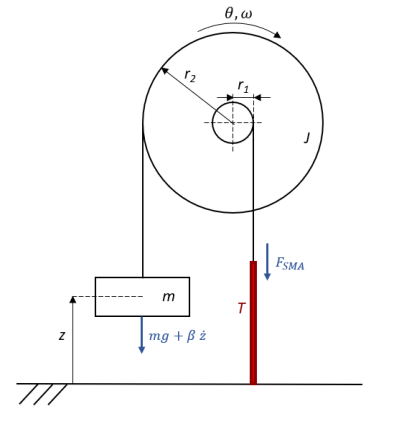
\includegraphics[scale = 0.6]{Immagini/progetto.png}
    \caption{Sistema di sollevamento con attuatore SMA}
    \label{fig:enter-label}
\end{figure}

Il progetto riguarda il controllo di un sistema di sollevamento con attuatore SMA, la cui dinamica viene descritta dalle seguenti equazioni differenziali 
%
\begin{subequations}\label{eq:system}

\begin{align}
	J\dot{\omega}& = F_{SMA} r_1 - (mg + \beta r_2\omega)r_2, 
	\\
	\mbox{con} \qquad F_{SMA}& = K_{max} \left(1-\frac{1}{1+\exp(k\frac{T-T_{avg}}{T_{diff}})}\right)(\ell - r_1 \theta)
\end{align}
\end{subequations}
%
dove $\theta(t)$ rappresenta la posizione angolare della puleggia e $\omega(t)$ rappresenta la velocità angolare. Gli altri parametri del sistema sono descritti come segue:

\begin{itemize}
    \item $r_1$: raggio interno puleggia
    \item $r_2$: raggio esterno puleggia
    \item $J$: momento di inerzia
    \item $m$: carico di massa
    \item $g$: costante di gravitazione universale
    \item $K_{max}$: rigidezza massima dell'attuatore
    \item $T$: temperatura (variabile di ingresso)
    \item $\beta$: coefficiente di attrito viscoso
\end{itemize}



\section{Espressione del sistema in forma di stato e calcolo del sistema linearizzato intorno ad una coppia di equilibrio}

Innanzitutto, esprimiamo il sistema~\eqref{eq:system} nella seguente forma di stato
%
\begin{subequations}
\begin{align}\label{eq:state_form}
	\dot{x} &= f(x,u)
	\\
	y &= h(x,u).
\end{align}
\end{subequations}
%
Pertanto, andiamo individuare lo stato $x$, l'ingresso $u$ e l'uscita $y$ del sistema. 
%
Supponiamo di potere misurare in ogni istante la posizione angolare $\theta$ della puleggia. Da ciò deriva la y scelta.
%
\begin{align*}
	x := \begin{bmatrix}\theta  \\ \dot{\theta}\end{bmatrix}, \quad u := T , \quad y := \theta.
\end{align*}
%
Coerentemente con questa scelta, ricaviamo dal sistema~\eqref{eq:system} la seguente espressione per le funzioni $f$ ed $h$
%
\begin{align*}
	f(x,u) &:= \dot{x} = \dot{\omega}= 
	\frac{K_{max}\left(1-\frac{1}{1+\exp\left(k\frac{u-T_{avg}}{T_{diff}}\right)}\right) (\ell-r_1x_1)r_1 - (mg + \beta  r_2  x_2) r_2}{J}
	\\
	h(x,u) &:= x_1
\end{align*}
%
Una volta calcolate $f$ ed $h$ esprimiamo~\eqref{eq:system} nella seguente forma di stato
%
\begin{subequations}\label{eq:our_system_state_form}
\begin{align}
	\begin{bmatrix}
		\dot{x}_1
		\\
		\dot{x}_2
	\end{bmatrix} &= 
        \begin{bmatrix}
            f_1(x,u) 
            \\
            f_2(x,u)
        \end{bmatrix} =
        \begin{bmatrix}
            x_2 
            \\
            \frac{K_{max}\left(1-\frac{1}{1+\exp\left(k\frac{u-T_{avg}}{T_{diff}}\right)}\right) (\ell-r_1x_1)r_1 - (mg + \beta  r_2  x_2) r_2}{J}
        \end{bmatrix} \label{eq:state_form_1}
	\\
	y &= h(x,u) = x_1
\end{align}
\end{subequations}
%
Per trovare la coppia di equilibrio $(x_e, u_e)$ di~\eqref{eq:our_system_state_form}, andiamo a risolvere il seguente sistema di equazioni
%
\begin{align}
	f(x_e,u_e) = 0  \\
	h(x_e,u_e) = 0 
\end{align}
%
dal quale otteniamo (considerando i dati forniti per i quali $\theta_e = \frac{\pi}{3}$)
%
\begin{align}
	x_e := 
        \begin{bmatrix}
	    \frac{\pi}{3} 
            \\
            0
	\end{bmatrix},  \quad u_e =  \frac{T_{diff}}{k} \cdot \log\left(\frac{1}{1 - \left(\frac{m \cdot g \cdot r_2}{K_{max} \cdot r1 \cdot (l - r_1 \cdot x_{1e})}\right)} - 1\right) + T_{avg}
 = 47.6735\label{eq:equilibirum_pair}
\end{align}

\vspace{0.2 cm}
%
Definiamo le variabili alle variazioni $\delta x$, $\delta u$ e $\delta y$ come 
%
\begin{align*}
	\delta x &= \Delta x, 
	\quad
	\delta u = \Delta u, 
	\quad
	\delta y = \Delta y.
\end{align*}
%
L'evoluzione del sistema espressa nelle variabili alle variazioni puo' essere approssimativamente descritta mediante il seguente sistema lineare
%
\begin{subequations}\label{eq:linearized_system}
\begin{align}
	\delta \dot{x} &= A\delta x + B\delta u
	\\
	\delta y &= C\delta x + D\delta u,
\end{align}
\end{subequations}
%
dove le matrici $A$, $B$, $C$ e $D$ vengono calcolate come
%
\begin{subequations}\label{eq:matrices}
\begin{align}
	A &= \begin{bmatrix}
	    \frac{\partial f_1(x,u)}{\partial x_1} & \frac{\partial f_1(x,u)}{x_2} \\
            \frac{\partial f_2(x,u) }{\partial x_1} & \frac{\partial f_2(x,u)}{ \partial x_2} 
	\end{bmatrix}_{x=x_e,u=u_e}
        & = & 
        \begin{bmatrix}
            0 & 1 \\
            \frac{K_{max}\cdot r_1^2 \cdot \left(\frac{1}{\exp\left(k\cdot\frac{u_e - T_{avg}}{T_{diff}}\right) + 1}\right) - 1}{J} &  -\frac{\beta\cdot r_2^2}{J}
        \end{bmatrix}
        & = &
        \begin{bmatrix}
                  0            &        1  
                  \\
                 -0.00011315   &        -0.0001684
        \end{bmatrix}
	\\
	B &= \begin{bmatrix}
	    \frac{\partial{f_1(x,u)}}{\partial u}  \\
            \frac{\partial{f_2(x,u)}}{\partial u} 
	\end{bmatrix}_{x=x_e,u=u_e}
        & = &
        \begin{bmatrix}
           0  \\
           \frac{K_{max}\cdot k \cdot r_1 \cdot \exp \left(k\frac{u_e - T_{avg}}{T_{diff}}\right) \cdot (l - r_1\cdot x_{1e})}{J \cdot T_{diff} \left(\exp\left(k\cdot\frac{u_e - T_{avg}}{T_{diff}}\right) + 1\right)^2}
        \end{bmatrix}
        & = &
        \begin{bmatrix}
            0 
            \\
            0.0056826
        \end{bmatrix}
	\\
	C &= \begin{bmatrix}
	    \frac{\partial{h(y,u)}}{\partial y}  & \frac{\partial{h(y,u)}}{\partial y} 
	\end{bmatrix}_{x=x_e,u=u_e}
        & = &
        \begin{bmatrix}
            1 & 0
        \end{bmatrix}
	\\
	D &= \begin{bmatrix} 
        \frac{\partial{h(x,u)}}{\partial u}  & \frac{\partial{h(x,u)}}{\partial u} 
        \end{bmatrix}_{x=x_e,u=u_e} 
        & = & \;0
\end{align}
\end{subequations}

Per quanto riguarda i calcoli delle matrici, questi ultimi sono stati in un primo momento effettuati a mano e successivamente controllati tramite la funzione \textbf{jacobian} di matlab con l'utilizzo di variabili \textbf{syms} per ottenere i risultati con i parametri.

\section{Calcolo Funzione di Trasferimento}

In questa sezione, andiamo a calcolare la funzione di trasferimento $G(s)$ dall'ingresso $\delta u$ all'uscita $\delta y$ mediante la seguente formula 
%
%
\begin{align}\label{eq:transfer_function}
G(s) = C (sI-A)^{-1} B + D = \frac{0.005685}{s^2 + 0.0001684 s + 8.299 \,\mbox{x}\, 10^{-5}}.
\end{align}
%
Dunque il sistema linearizzato~\eqref{eq:linearized_system} è caratterizzato dalla funzione di trasferimento~\eqref{eq:transfer_function} con 2 poli complessi coniugati $p_1 =  -0.0001 + 0.0091 i$ , $p_2 =  -0.0001 - 0.0091 i$ e nessuno zero. In Figura 2 mostriamo il corrispondente diagramma di Bode. 

\begin{figure} [htp]
    \centering
    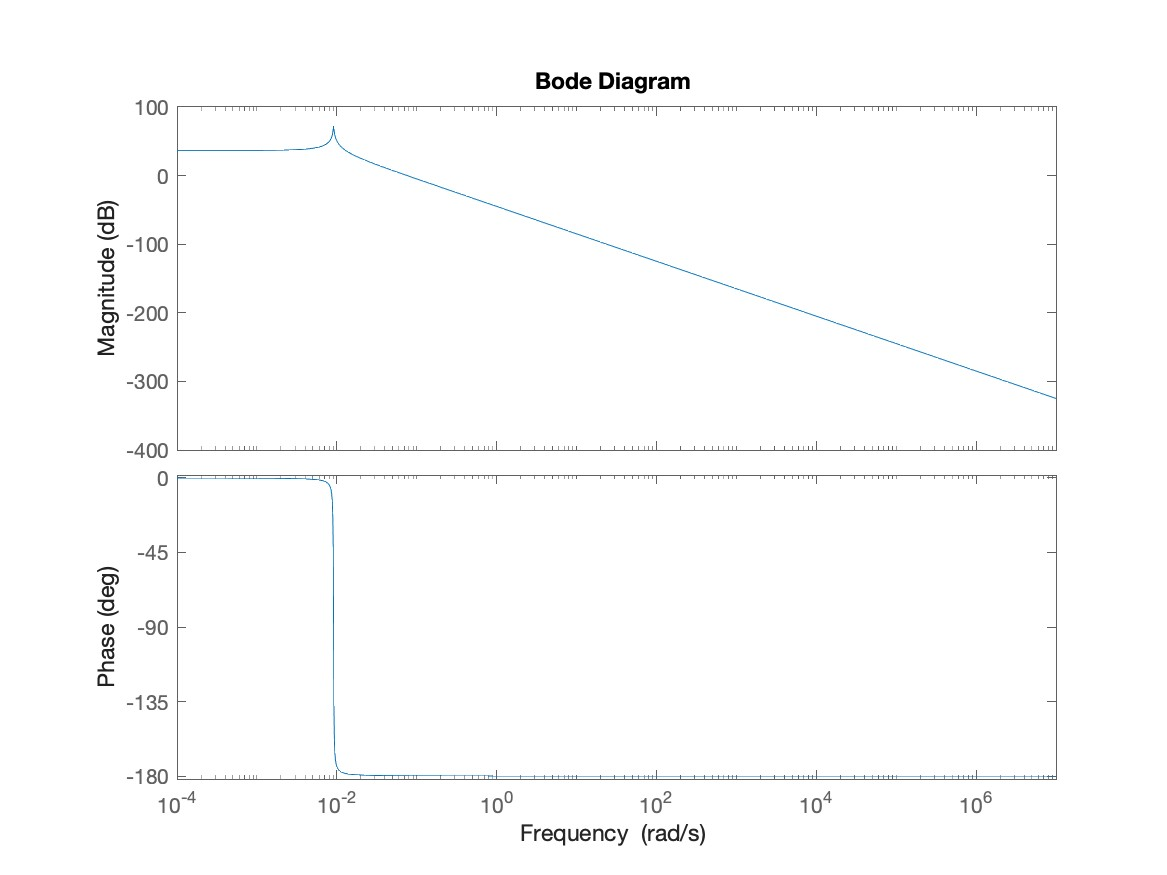
\includegraphics[scale = 0.28]{Immagini/Bode_GG.jpg}
    \caption{Diagramma di Bode $G(s)$}
    \label{fig:enter-label}
\end{figure}

\vspace{10 cm}

\section{Mappatura specifiche del regolatore}
\label{sec:specifications}

Le specifiche da soddisfare sono
\begin{itemize}
	\item[1)] errore a regime $|e_{\infty}| \le e^* = 0.01$ in risposta a un gradino $w(t) = 1(t)$ e $d(t) = 1(t)$
	\item[2)] margine di fase \textbf{$M_f \ge 40 \degree$}
	\item[3)] sovraelongazione percentuale massima $S\% \le 7\%$
        \item[4)] tempo di assestamento a $T_{a,\epsilon} = 0.1s$, con $\epsilon\% = 5\%$
        \item[5)] disturbo sull'uscita $d(t)$, con banda nel range di pulsazioni $[0,0.05]$, abbattuto di almeno 50 dB
        \item[6)] disturbo di misura $N(t)$, con banda nel range di pulsazioni $[10^4,10^6]$, abbattuto di almeno 100 dB
\end{itemize}
%
Andiamo ad effettuare la mappatura punto per punto le specifiche richieste. 

\subsection{\textbf{Vincolo sulla sovraelongazione $S\%$}} 
Il vincolo sulla sovraelongazione viene realizzato agendo sul \textbf{margine di fase}. \\

\begin{lstlisting}[
frame=single,
numbers=left,
style=Matlab-Pyglike]
Mf_esp = 40

% calcolo specifiche S% -> margine di fase
xi_star = abs(log(S_star/100))/sqrt(pi^2 + log(S_star/100)^2);
Mf = max(xi_star*100,Mf_esp);
\end{lstlisting}

Otteniamo un margine di fase pari a 64.6082. 

\subsection{\textbf{Specifica sul tempo di assestamento $T_{a,5}$}}
Per quanto concerne la specifica sul tempo di assestamento, agiamo sulla pulsazione critica minima $\omega_c$. \\ 

\begin{lstlisting}[
frame=single,
numbers=left,
style=Matlab-Pyglike]
T_star = 0.1

% usiamo 300 in quanto abbiamo ragionato al 5%
omega_Ta_min = 1e-6;
omega_Ta_max = 300/(Mf * T_star)
omega_c_min = omega_Ta_max
\end{lstlisting}

Otteniamo una $\omega_{c_{min}} = 46.4337$.

\subsection{\textbf{Patch specifiche disturbo sull'uscita}}


\begin{lstlisting}[
frame=single,
numbers=left,
style=Matlab-Pyglike]
A_d = 50;

% Per la specifica della pulsazione minima del disturbo sull'uscita uso un valore molto vicino allo 0 in quanto log(0) non esiste
omega_d_min = 1e^-1;
omega_d_max = 0.05;
Bnd_d_x = [omega_d_min; omega_d_max; omega_d_max; omega_d_min];
Bnd_d_y = [A_d; A_d; -150; -150];
patch(Bnd_d_x, Bnd_d_y,'r','FaceAlpha',0.2,'EdgeAlpha',0);

\end{lstlisting}

\subsection{\textbf{Patch specifiche disturbo di misura}}

\begin{lstlisting}[
frame=single,
numbers=left,
style=Matlab-Pyglike]
A_n = 100;
omega_n_min = 1e5;
omega_n_max = 1e7;
Bnd_n_x = [omega_n_min; omega_n_max; omega_n_max; omega_n_min];
Bnd_n_y = [-A_n; -A_n; 100; 100];
patch(Bnd_n_x, Bnd_n_y,'y','FaceAlpha',0.2,'EdgeAlpha',0);
\end{lstlisting}

\subsection{\textbf{Patch specifiche sovraelongazione $S\%$}}

\begin{lstlisting}[
frame=single,
numbers=left,
style=Matlab-Pyglike]
omega_c_min = omega_Ta_max;
omega_c_max = omega_n_min;
phi_up = Mf - 180;
phi_low = -360; % lower bound per il plot
Bnd_Mf_x = [omega_c_min; omega_c_max; omega_c_max; omega_c_min];
Bnd_Mf_y = [phi_up; phi_up; phi_low; phi_low];
patch(Bnd_Mf_x, Bnd_Mf_y,'g','FaceAlpha',0.2,'EdgeAlpha',0);

\end{lstlisting}

\subsection{\textbf{Patch specifiche tempo di assestamento}}

\begin{lstlisting}[
frame=single,
numbers=left,
style=Matlab-Pyglike]
omega_Ta_min = 1e-6;
omega_Ta_max = 300/(Mf * T_star)
Bnd_Ta_x = [omega_Ta_min; omega_Ta_max; omega_Ta_max; omega_Ta_min];
Bnd_Ta_y = [0; 0; -150; -150];
patch(Bnd_Ta_x, Bnd_Ta_y,'b','FaceAlpha',0.2,'EdgeAlpha',0);

\end{lstlisting}

Pertanto, in Figura 3, mostriamo il diagramma di Bode della funzione di trasferimento $G(s)$ con le zone proibite emerse dalla mappatura delle specifiche.

\begin{figure} [!htp]
    \centering
    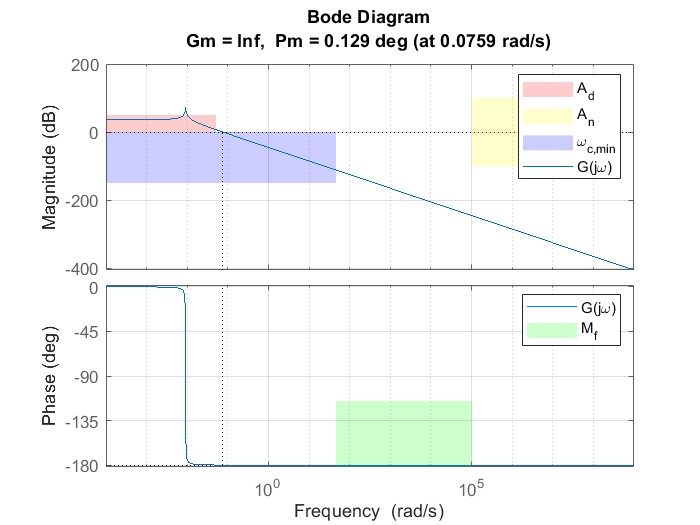
\includegraphics[scale = 0.45]{Immagini/BODE/bode_G.jpg}
    \caption{Diagramma di Bode $G(s)$ con specifiche mappate}
    \label{fig:enter-label}
\end{figure}

\vspace{12cm}

\section{Sintesi del regolatore statico}
\label{sec:static_regulator}

In questa sezione progettiamo il regolatore statico $R_s(s)$ partendo dalle analisi fatte in sezione~\ref{sec:specifications}.

\subsection{\textbf{Considerazione sulla realizzazione}}
Di seguito le considerazioni fatte sull'errore a regime. Trattandosi di una specifica che non pone un vincolo di errore a regime nullo ($|e_{\infty}| = 0$) e considerando la generica forma del regolatore statico $\frac{u_s}{s^k}$, avevamo la possibilità di scegliere tra $R(s) = \mu_s \ge \mu^*$, dove $\mu^* = \frac{D^* + W^*}{e^*}$ e $R(s) = \frac{\mu_s}{s}$.

\vspace{0.2 cm}

Abbiamo scelto di considerare un guadagno $\mu_s \ge \mu^*$, dove oltre al calcolo di $\mu^*$ abbiamo considerato anche la specifica imposta dal disturbo $d(t)$, andando a scegliere come regolatore statico il vincolo più stringente (espresso dalla scelta del massimo nel codice matlab).

\vspace{0.2 cm}

\begin{lstlisting}[
frame=single,
numbers=left,
style=Matlab-Pyglike]
mu_s_error = (WW + DD)/e_star/abs(evalfr(GG,j*0));
G_omega_d_max = abs(evalfr(GG,j*omega_d_max));
mu_s_d = 10^(A_d/20)/G_omega_d_max;
R_s = max(mu_s_error,mu_s_d)
\end{lstlisting}

Il risultato dei due guadagni è stato il seguente:
\vspace{0.2 cm}
$$\mu_s = \frac{\frac{WW + DD}{e^*}}{G(0)} = 2.9198, \qquad \mu_{s_d} = \frac{10^{\frac{A_d}{20}}}{G(\omega_{d_{max}})} = 134.4563$$ 
Dunque, definiamo la funzione estesa $G_e(s) = R_s(s)G(s)$ e, in Figura 4, mostriamo il suo diagramma di Bode per verificare se e quali zone proibite vengono attraversate.




\begin{align}
R_s & = 134.4563
\\
G_e(s) & =  GG *R_s = \frac{0.005685}{s^2 + 0.0001684 s + 8.299 \,\mbox{x}\, 10^{-5}} * 134.4563 =   \frac{0.7643}{s^2 + 0.0001684 s + 8.299\,\mbox{x}10^{-5}}
\end{align}

Da Figura 4, emerge

\begin{figure} [!h]
    \centering
    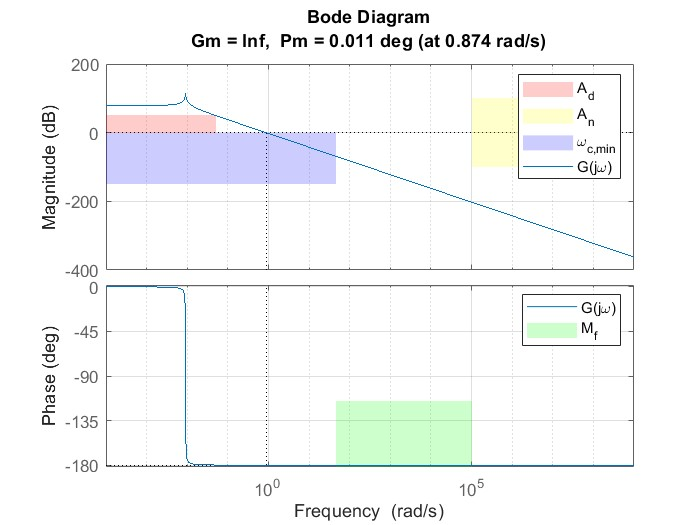
\includegraphics[scale = 0.45]{Immagini/BODE/bode_Ge.jpg}
    \caption{Diagramma di Bode $G_e(s)$ con specifiche mappate}
    \label{fig:enter-label}
\end{figure}


\section{Sintesi del regolatore dinamico}

In questa sezione, progettiamo il regolatore dinamico $R_d(s)$. 
%
Dalle analisi fatte in Sezione~\ref{sec:static_regulator}, notiamo di essere nello Scenario di tipo B. Dunque, progettiamo $R_d(s)$ ricorrendo ad una rete anticipatrice.

Per realizzarla, partiamo dalla formula generale che la descrive: 
$$R_d(s) = \frac{1+\tau s}{1+\alpha \tau s} \qquad 0 < \alpha < 1$$. 

Per il calcolo di $\alpha \tau$ e $\tau$ facciamo uso delle formule di inversione: 
$$\tau = \frac{M^*-\cos\varphi^*}{\omega_c^*\sin\varphi^*}, \qquad \alpha \tau = \frac{\cos \varphi^* - \frac{1}{M^*}}{\omega_c^*\sin\varphi^*}$$.

Come mostrato nel codice matlab sottostante, consideriamo un margine di fase di partenza pari a quello calcolato nella mappatura delle specifiche con l'aggiunta di un valore 5 per essere più conservativi. 

\vspace{1cm}

Per quanto concerne $\omega_c^*$ il valore imposto è 200.

\vspace{1cm}

\begin{lstlisting}[
frame=single,
numbers=left,
style=Matlab-Pyglike]
% prendiamo margine + 5 per essere conservativi
Mf_star = Mf + 5;
omega_c_star = 200;

% modulo della G estesa in omega_c_star
mag_omega_c_star_dB = abs(evalfr(GG_e,j*omega_c_star));

% fase della G estesa in omega_c_star
arg_omega_c_star = rad2deg(angle(evalfr(GG_e,j*omega_c_star)));

M_star = 1/mag_omega_c_star_dB;
phi_star = Mf_star - 180 - arg_omega_c_star;

tau = (M_star-cos(phi_star*pi/180))/(omega_c_star*sin(phi_star*pi/180));
alpha_tau = (cos(phi_star*pi/180) - 1/M_star)/(omega_c_star*sin(phi_star*pi/180));
alpha = alpha_tau / tau;
R_d = (1 + tau*s)/(1 + alpha * tau*s);
L = R_d*G_e;
\end{lstlisting}

\vspace{1 cm}

In Figura 5, mostriamo il diagramma di Bode della funzione d'anello $L(s) = R_d(s) G_e(s)$

\begin{figure} [!h]
    \centering
    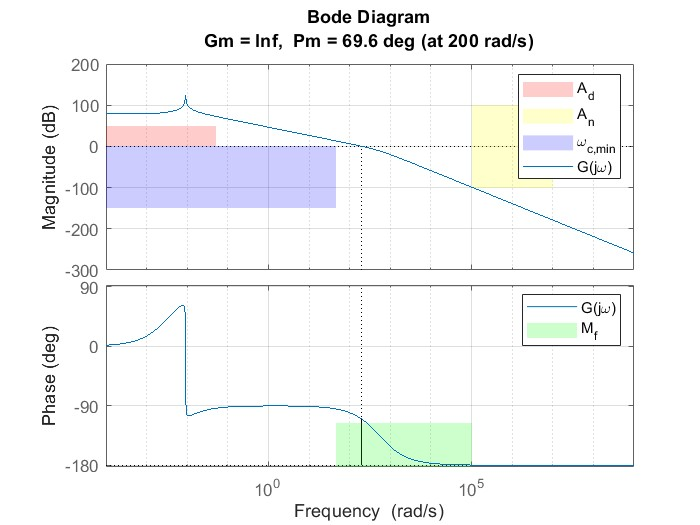
\includegraphics[scale = 0.55]{Immagini/BODE/bode_N_P.jpg}
    \caption{Diagramma di Bode $L$}
    \label{fig:enter-label}
\end{figure}

\vspace{5cm}

Possiamo notare come non vengano rispettate tutte le specifiche. In particolare, la funzione non rispetta la specifica sul \textbf{disturbo di misura}.

\vspace{0.4cm}

\begin{figure} [!h]
    \centering
    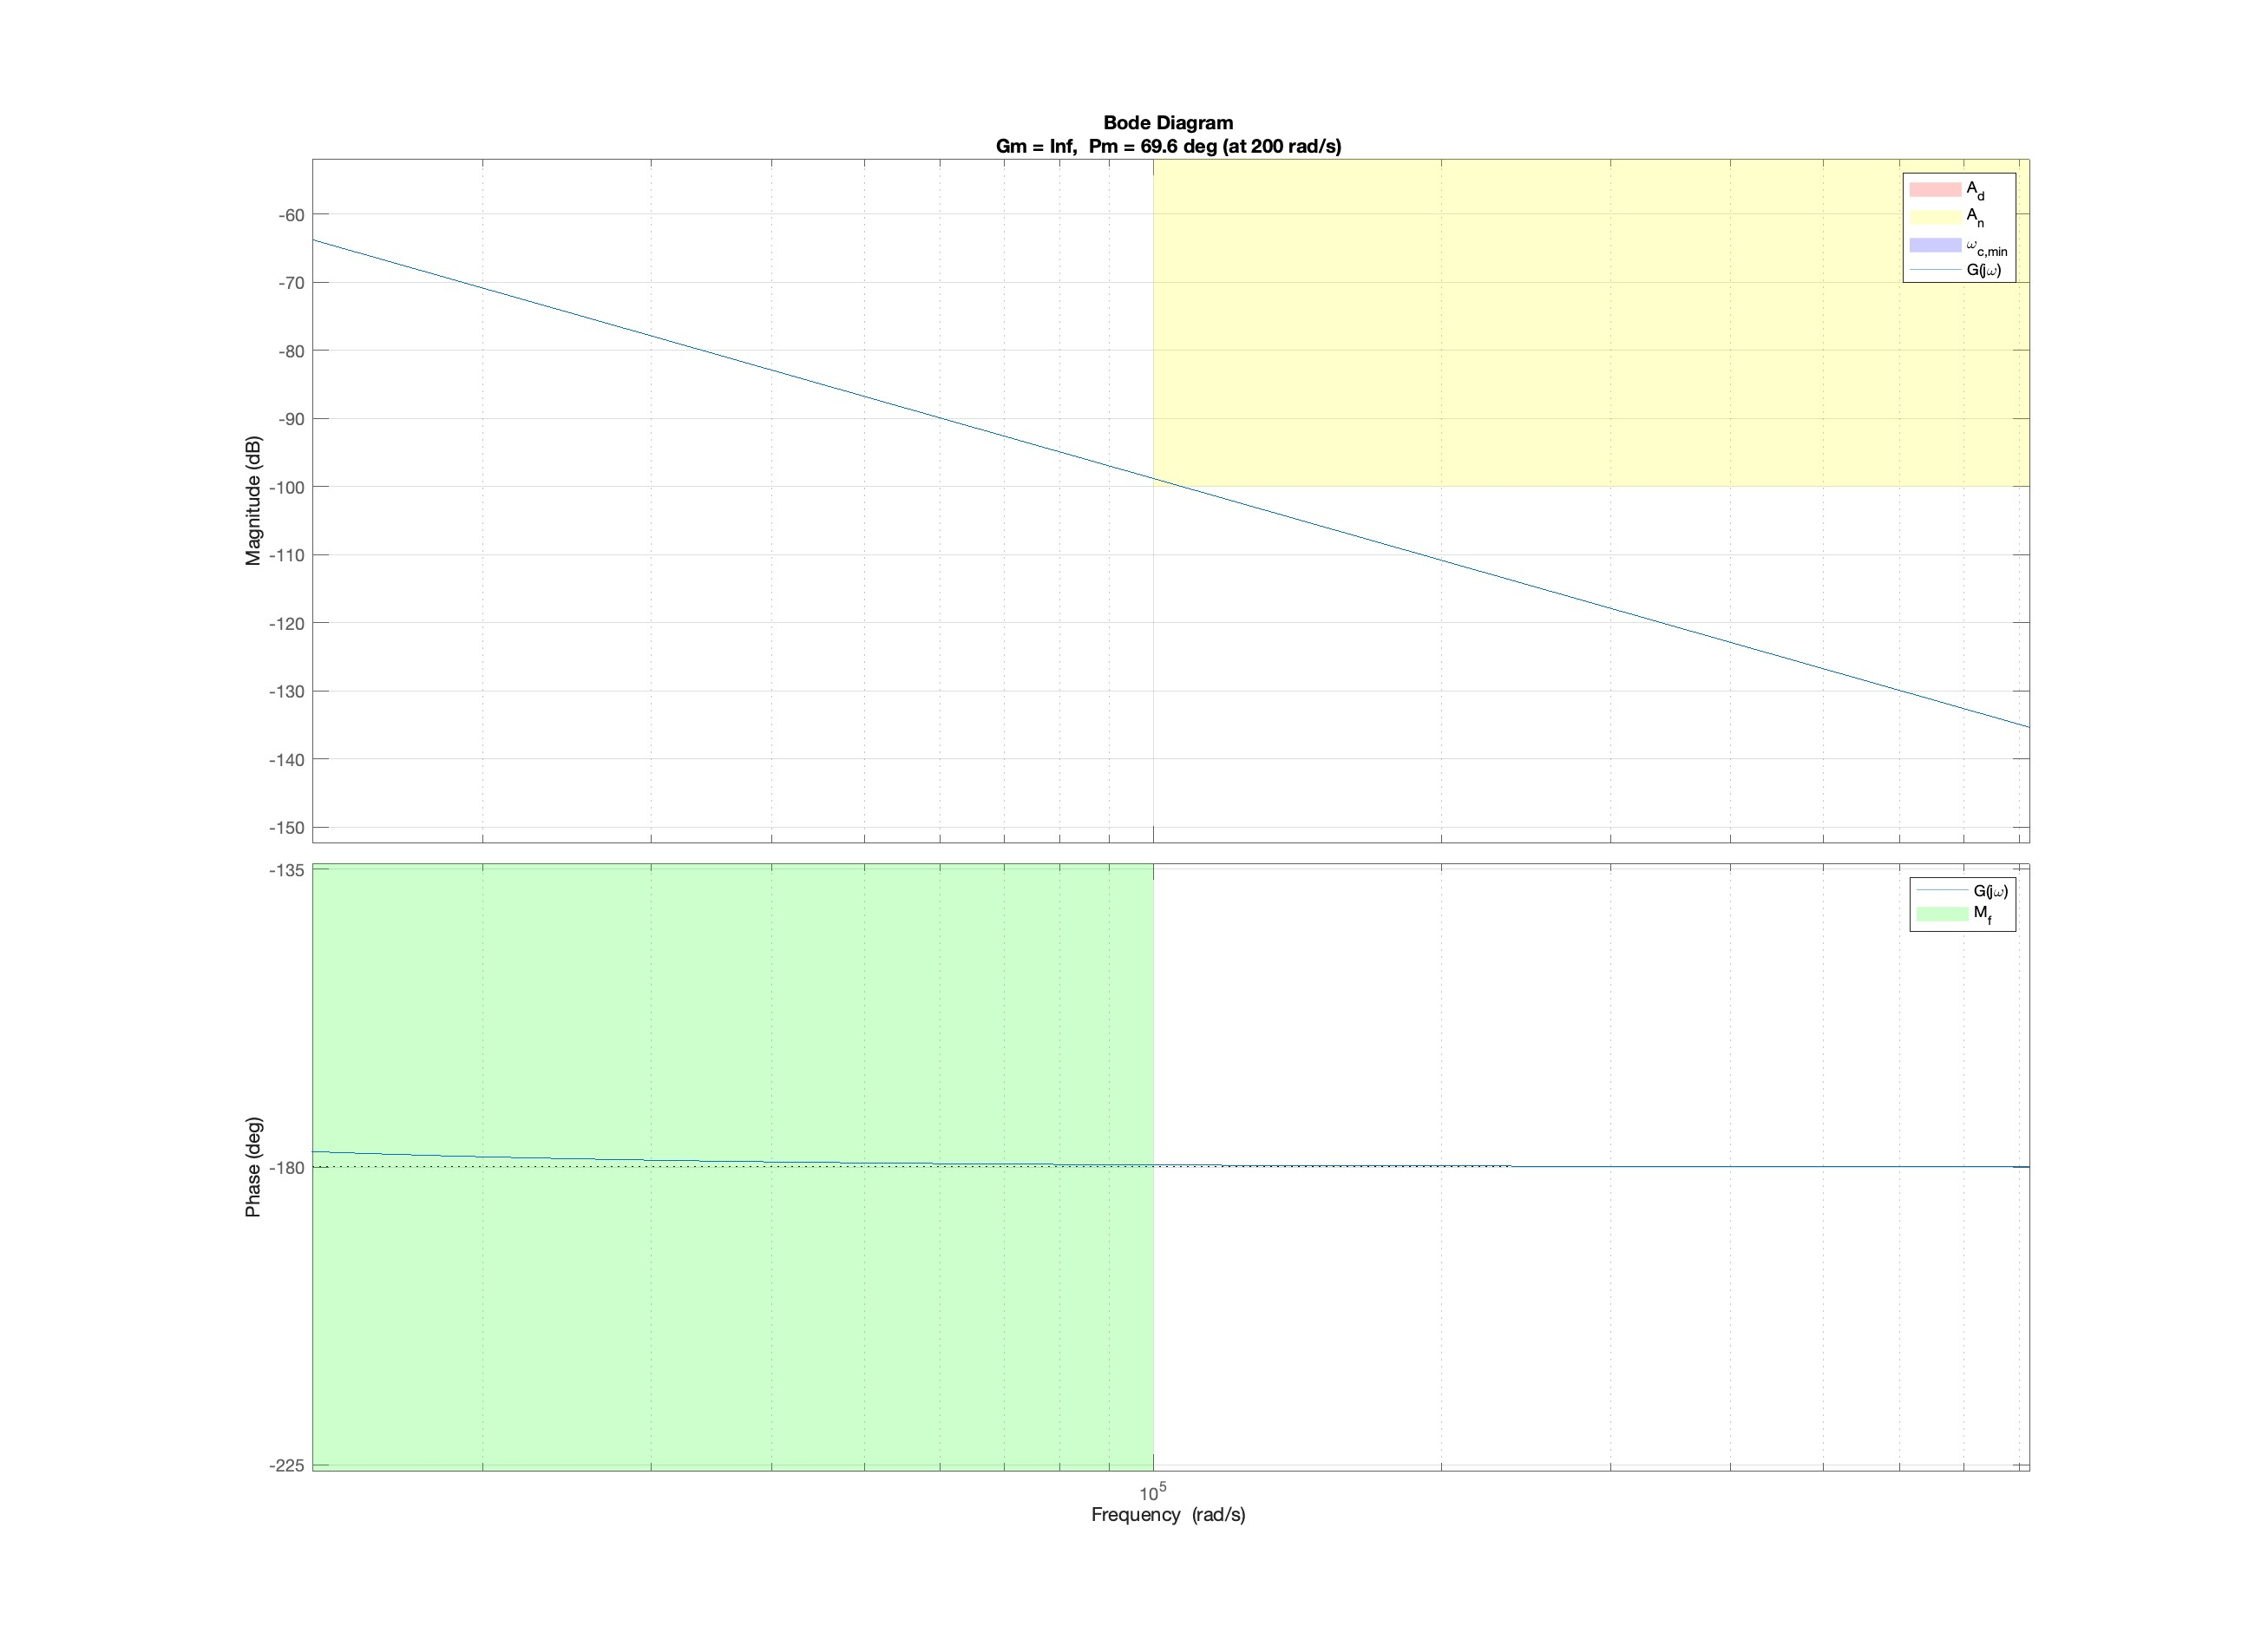
\includegraphics[scale = 0.15]{Immagini/LL_dettaglio.jpg}
    \caption{Dettaglio diagramma di Bode $L$}
    \label{fig:enter-label}
\end{figure}

\vspace{5cm}

Al fine di evitare che la funzione attraversi la zona, usiamo un polo in alta frequenza (nello specifico a $\omega = 4000$. Questo comporta un abbassamento di 20dB/dec della funzione in termini di diagramma delle ampiezze e un abbassamento della fase di 90°.

Polo inserito : $$\frac{1}{1 + \frac{s}{4000}}$$

Per aggiungere l'effetto del polo al regolatore lo moltiplichiamo per la rete anticipatrice calcolata.

\vspace{1.5cm}

\begin{lstlisting}[
frame=single,
numbers=left,
style=Matlab-Pyglike]
% polo ad alta frequenza
R_high_frequency = 1/(1 + s/4e3);

RR_d = (1 + tau*s)/(1 + alpha * tau*s)*R_high_frequency;

% funzione di anello
LL = R_d*G_e; 
\end{lstlisting}

\vspace{1cm}

In Figura 7, mostriamo il diagramma di Bode della funzione d'anello $L(s) = R_d(s) G_e(s)$

\begin{figure} [!h]
    \centering
    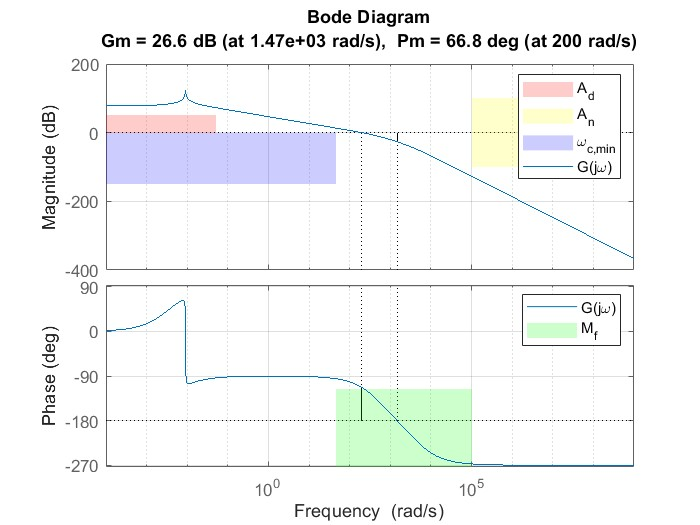
\includegraphics[scale = 0.7]{Immagini/BODE/bode_L.jpg}
    \caption{Diagramma di Bode $L$}
    \label{fig:enter-label}
\end{figure}

\vspace{4 cm}

In Figura 8, mostriamo la risposta al gradino della funzione d'anello $L(s)$. Il gradino considerato in base alla specifica è $1(t)$ e la funzione \textbf{step} è stata applicata sulla funzione di sensitività complementare: $$F(s) = \frac{R(s)G(s)}{1+R(s)G(s)} = \frac{L(s)}{1+L(s)}$$

\begin{figure} [!h]
    \centering
    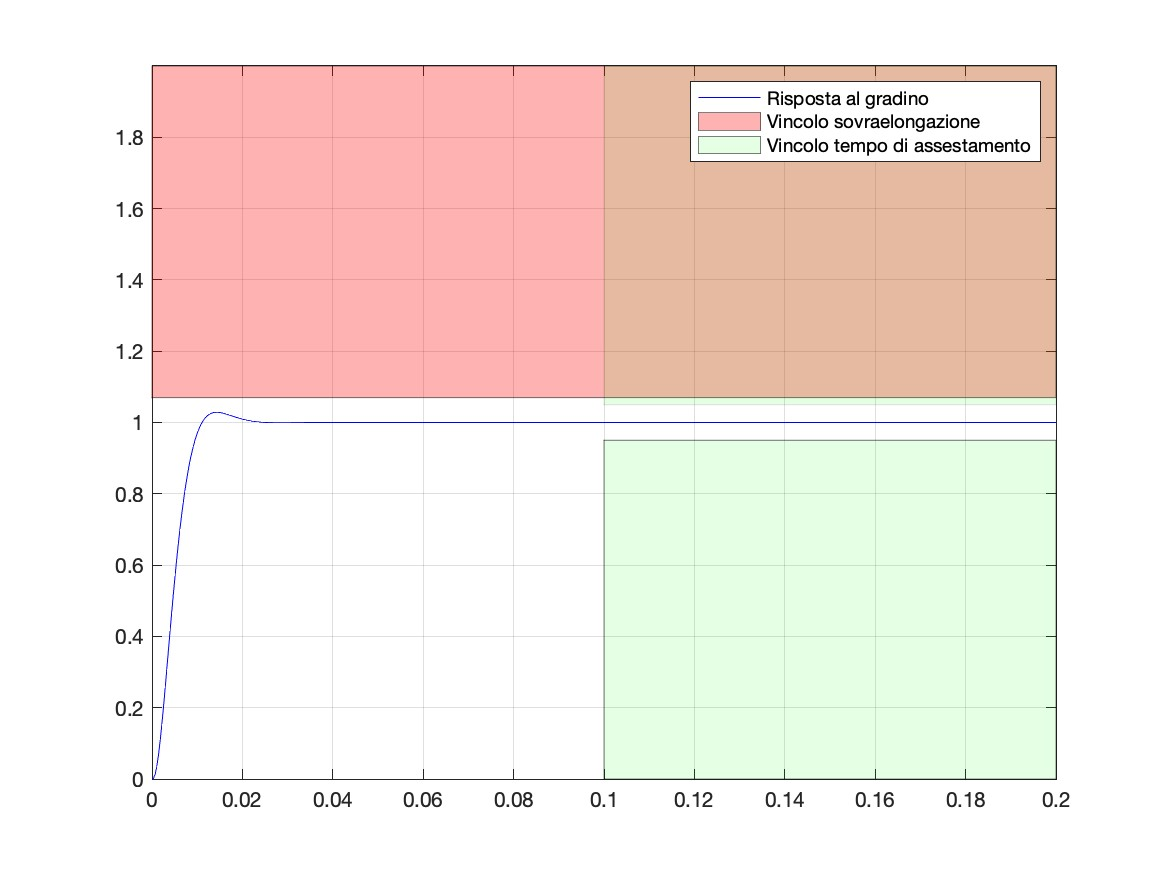
\includegraphics[scale = 0.4]{Immagini/Step_1.jpg}
    \caption{Risposta al gradino di $L$}
    \label{fig:enter-label}
\end{figure}

\vspace{19cm}

\section{Test sul sistema linearizzato}

In questa sezione, testiamo l'efficacia del controllore progettato sul sistema linearizzato con $w(t) = 1(t), d(t) = \sum_{k=1}^3 \sin(0.01kt)$ e $n(t) = \sum_{k=1}^3\sin(10^4kt)$

\subsection{\textbf{Test con $d(t) = \sum_{k=1}^3\sin(0.01kt)$}}

\begin{figure} [!h]
    \centering
    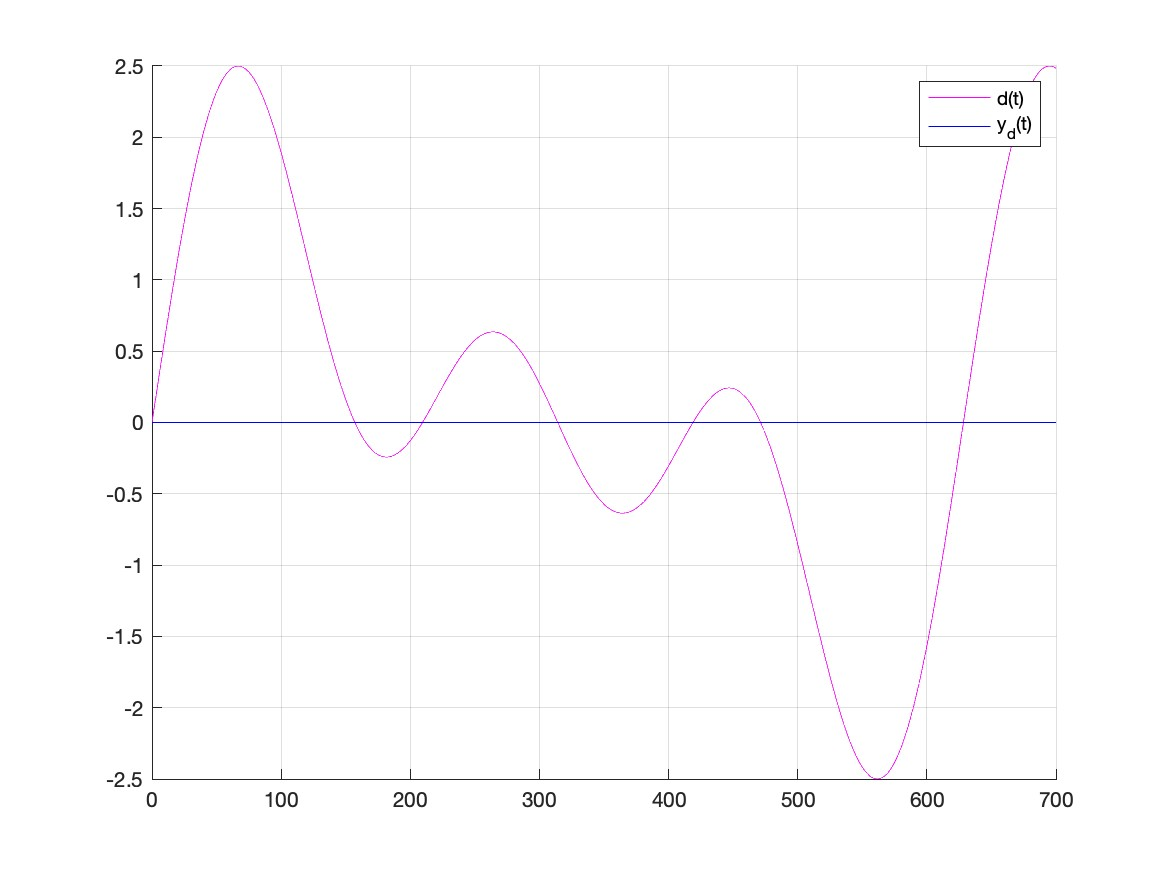
\includegraphics[scale = 0.25]{Immagini/Disturbo_uscita.jpg}
    \caption{Comportamento sistema linearizzato con disturbo sull'uscita}
    \label{fig:enter-label}
\end{figure}

\subsection{\textbf{Test con $n(t) = \sum_{k=1}^3\sin(10^4kt)$}}


\begin{figure} [!h]
    \centering
    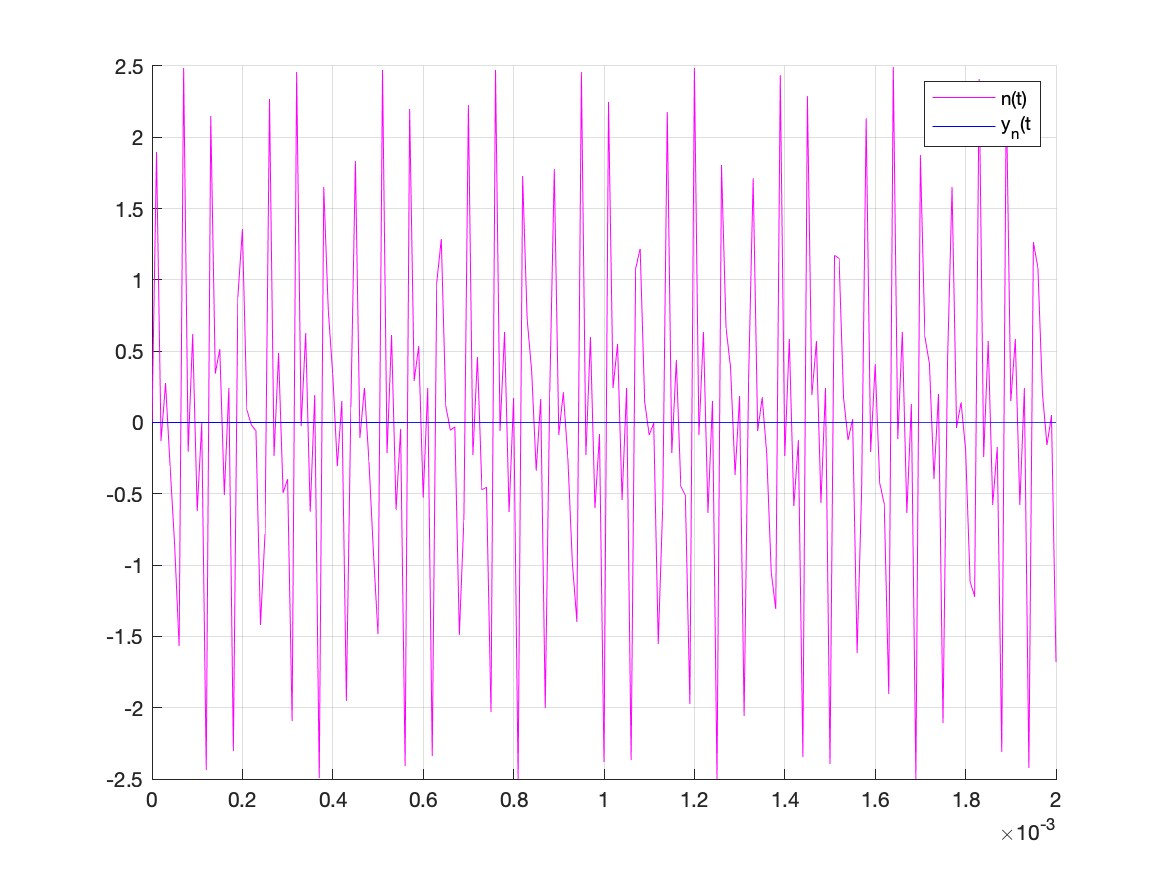
\includegraphics[scale = 0.25]{Immagini/Disturbo_misura.jpg}
    \caption{Comportamento sistema linearizzato con disturbo di misura}
    \label{fig:enter-label}
\end{figure}

\subsection{Simulink linearizzato}

Abbiamo considerato lo schema a blocchi del sistema linearizzato e valutato la risposta avendo come $x$ il punto di equilibrio. Specifiche sui blocchi inseriti:
\begin{itemize}
    \item gradino all'interno del blocco \textbf{step}: $WW = 1$ con step time = 0 per simulare il gradino
    \item ampiezza e frequenza del blocco relativo al \textbf{disturbo di misura}: ampiezza di 0.01, frequenza di 1000 $\frac{rad}{s}$
\end{itemize}

\vspace{0.2cm}

\textbf{Sistema linearizzato}
\begin{figure} [!h]
    \centering
    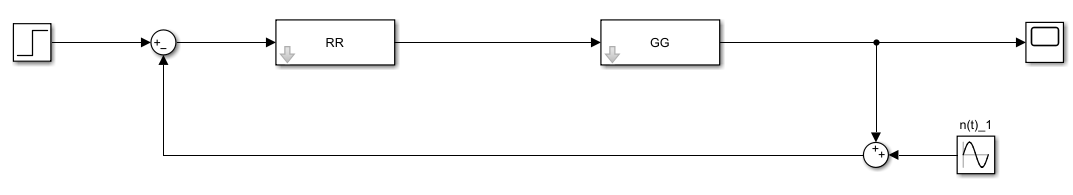
\includegraphics[scale = 0.6]{Simulink/Sim_lin_disturbi.png}
    \caption{Sistema linearizzato Simulink}
    \label{fig:enter-label}
\end{figure}

\vspace{1cm}

\textbf{Risposta linearizzato}

\begin{figure} [!h]
    \centering
    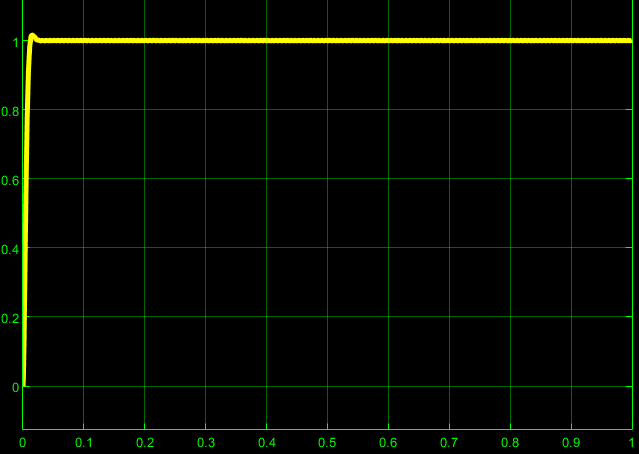
\includegraphics[scale = 0.9]{Immagini/linearizzato_risposta.png}
    \caption{Risposta sistema linearizzato}
    \label{fig:enter-label}
\end{figure}

\vspace{20 cm}

\section{Test sul sistema non lineare}

In questa sezione, testiamo l'efficacia del controllore progettato sul modello non lineare con ingresso $x$ che coincide con il suo punto di equilibrio.Specifiche sui blocchi inseriti:

\begin{itemize}
    \item gradino all'interno del blocco \textbf{step}: $WW = 1$ con step time = 0 per simulare il gradino
    \item ampiezza e frequenza del blocco relativo al \textbf{disturbo di misura}: ampiezza di 0.01, frequenza di 1000 $\frac{rad}{s}$
    \item ampiezza e frequenza del blocco relativo al \textbf{disturbo sull'uscita}:
    ampiezza di 0.01, frequenza di 0.01 $\frac{rad}{s}$
\end{itemize}

\vspace{0.2cm}

\textbf{Sistema non linearizzato}
\begin{figure} [!h]
    \centering
    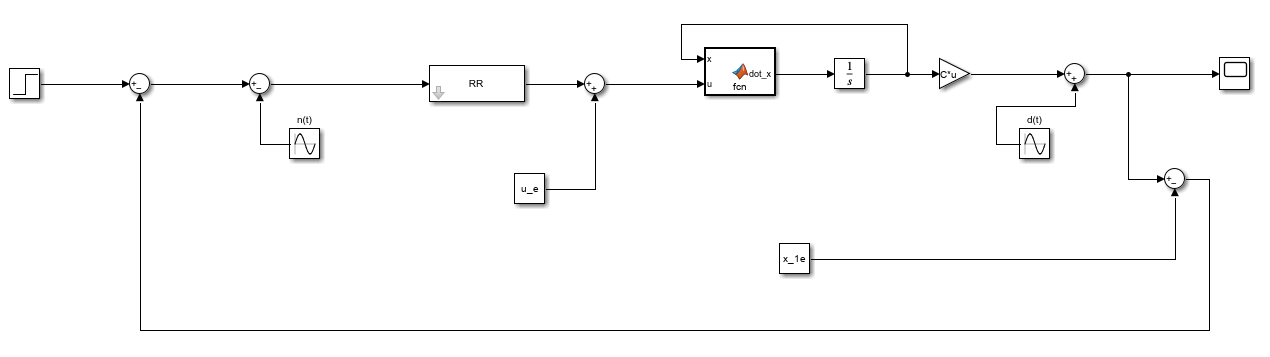
\includegraphics[scale = 0.5]{Simulink/Sim_non_lin_disturbi.png}
    \caption{Sistema non linearizzato Simulink}
    \label{fig:enter-label}
\end{figure}

\vspace{0.3cm}

\textbf{Risposta non linearizzato}

\begin{figure} [!h]
    \centering
    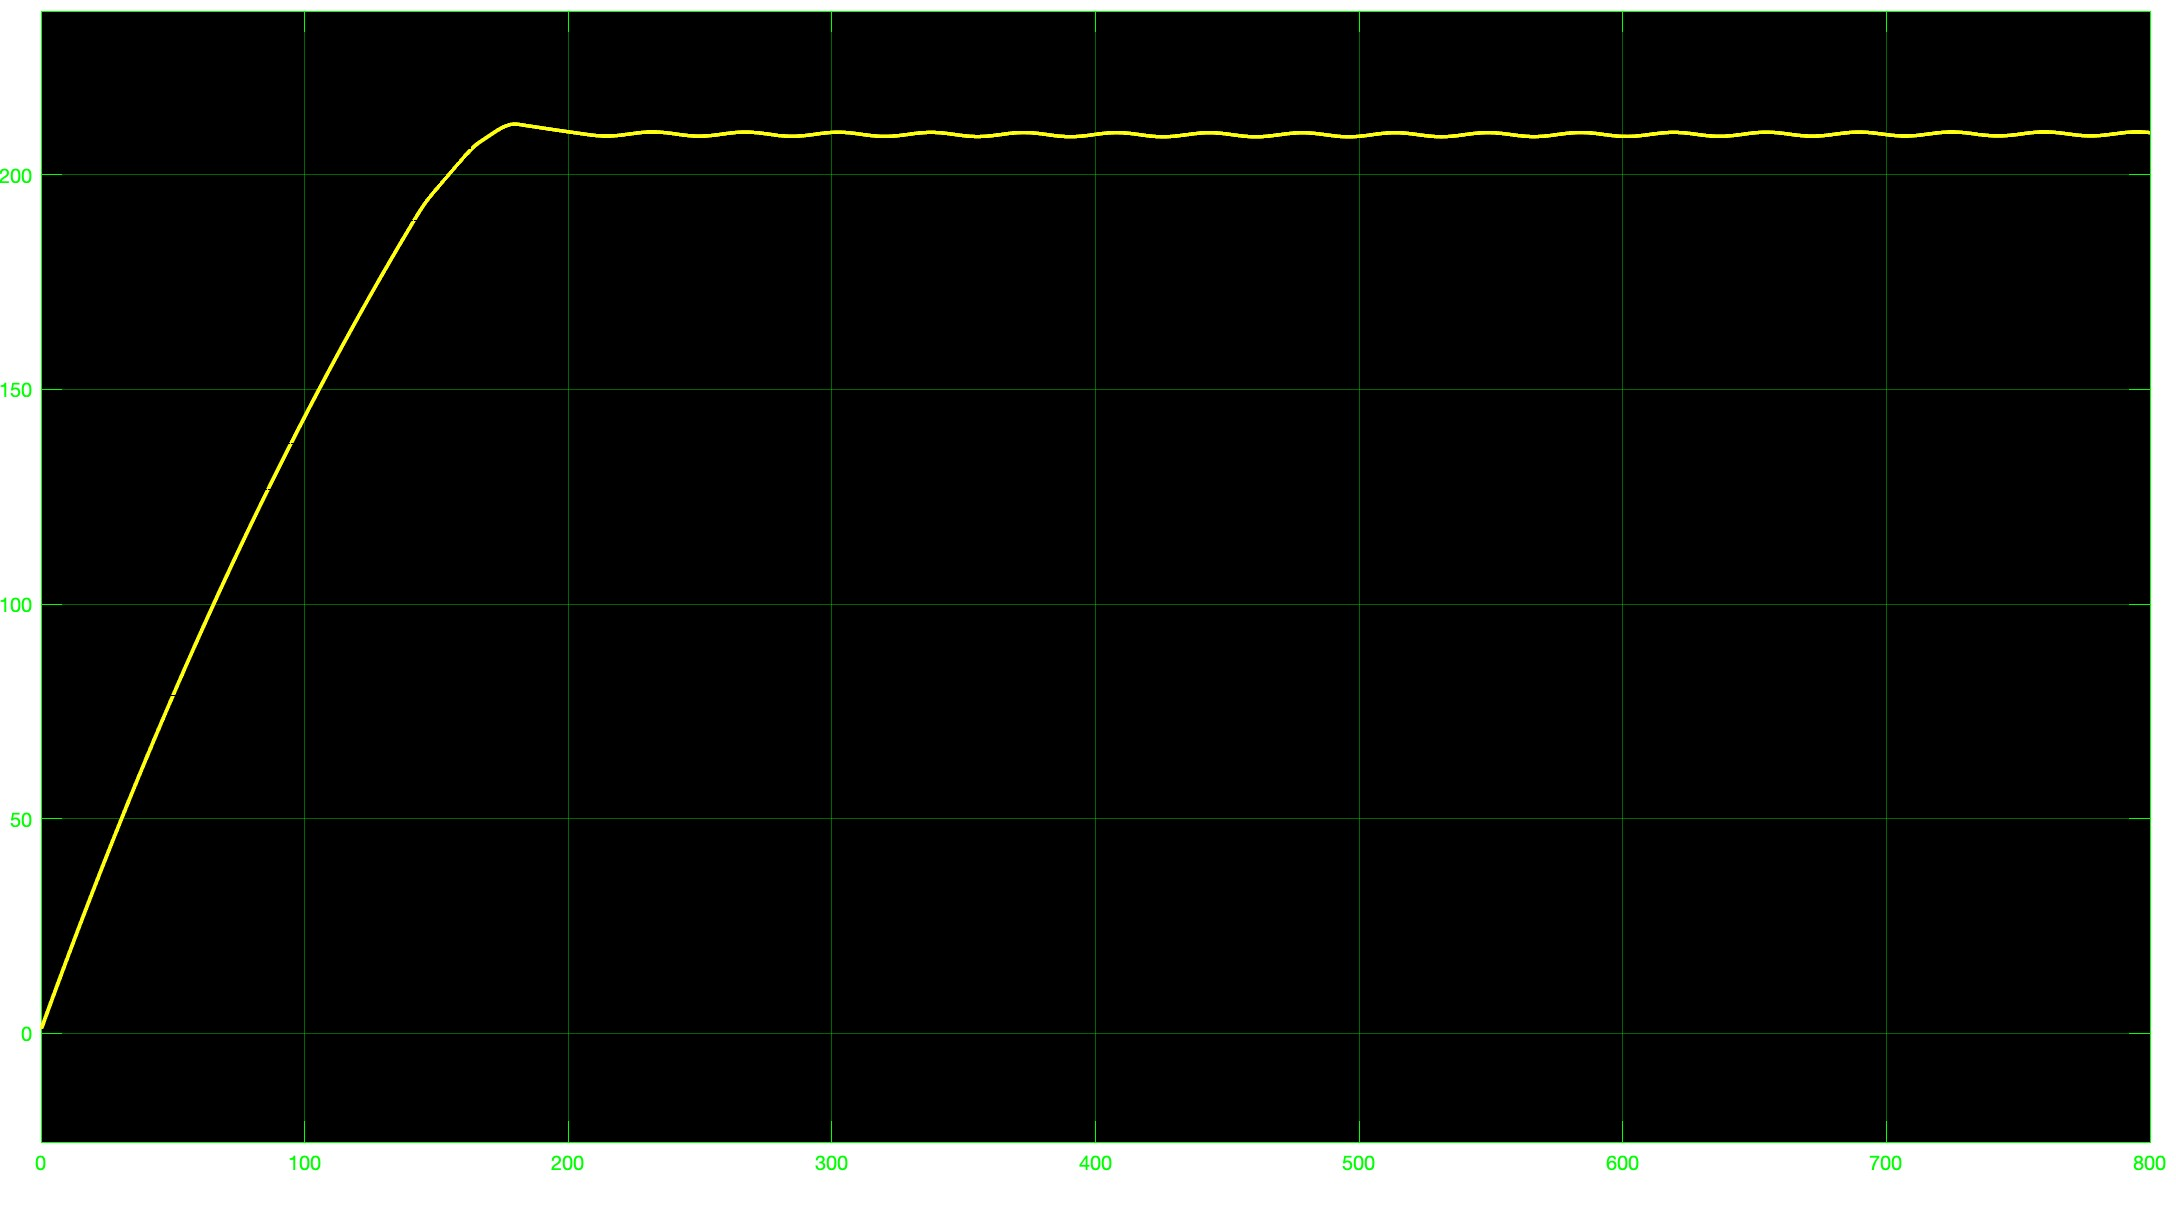
\includegraphics[scale = 0.22]{Step_nonLineare/Step1_noLin.jpg}
    \caption{Risposta sistema non linearizzato}
    \label{fig:enter-label}
\end{figure}



\section{Punti opzionali}

\subsection{Secondo punto}

Ci focalizziamo sulla risposta del sistema non lineare quando sottoposto a un riferimento costante, $\theta(t)$ $\equiv$ $\theta_e$ . L'obiettivo principale consiste nell'esplorare il range di condizioni iniziali dello stato del sistema in anello chiuso, concentrandoci sull'intorno del punto di equilibrio. Questa analisi mira a fornire una comprensione dettagliata di come variazioni iniziali nello stato del sistema possano influenzare la convergenza dell'uscita del sistema a $h(x_e, u_e)$. Avendo $x_1 = \theta_e = \frac{\pi}{3}$ come riferimento, agiamo sul valore di $x_2$, facendolo variare per vedere come cambia la risposta.

\begin{figure}[!h]
    \centering
    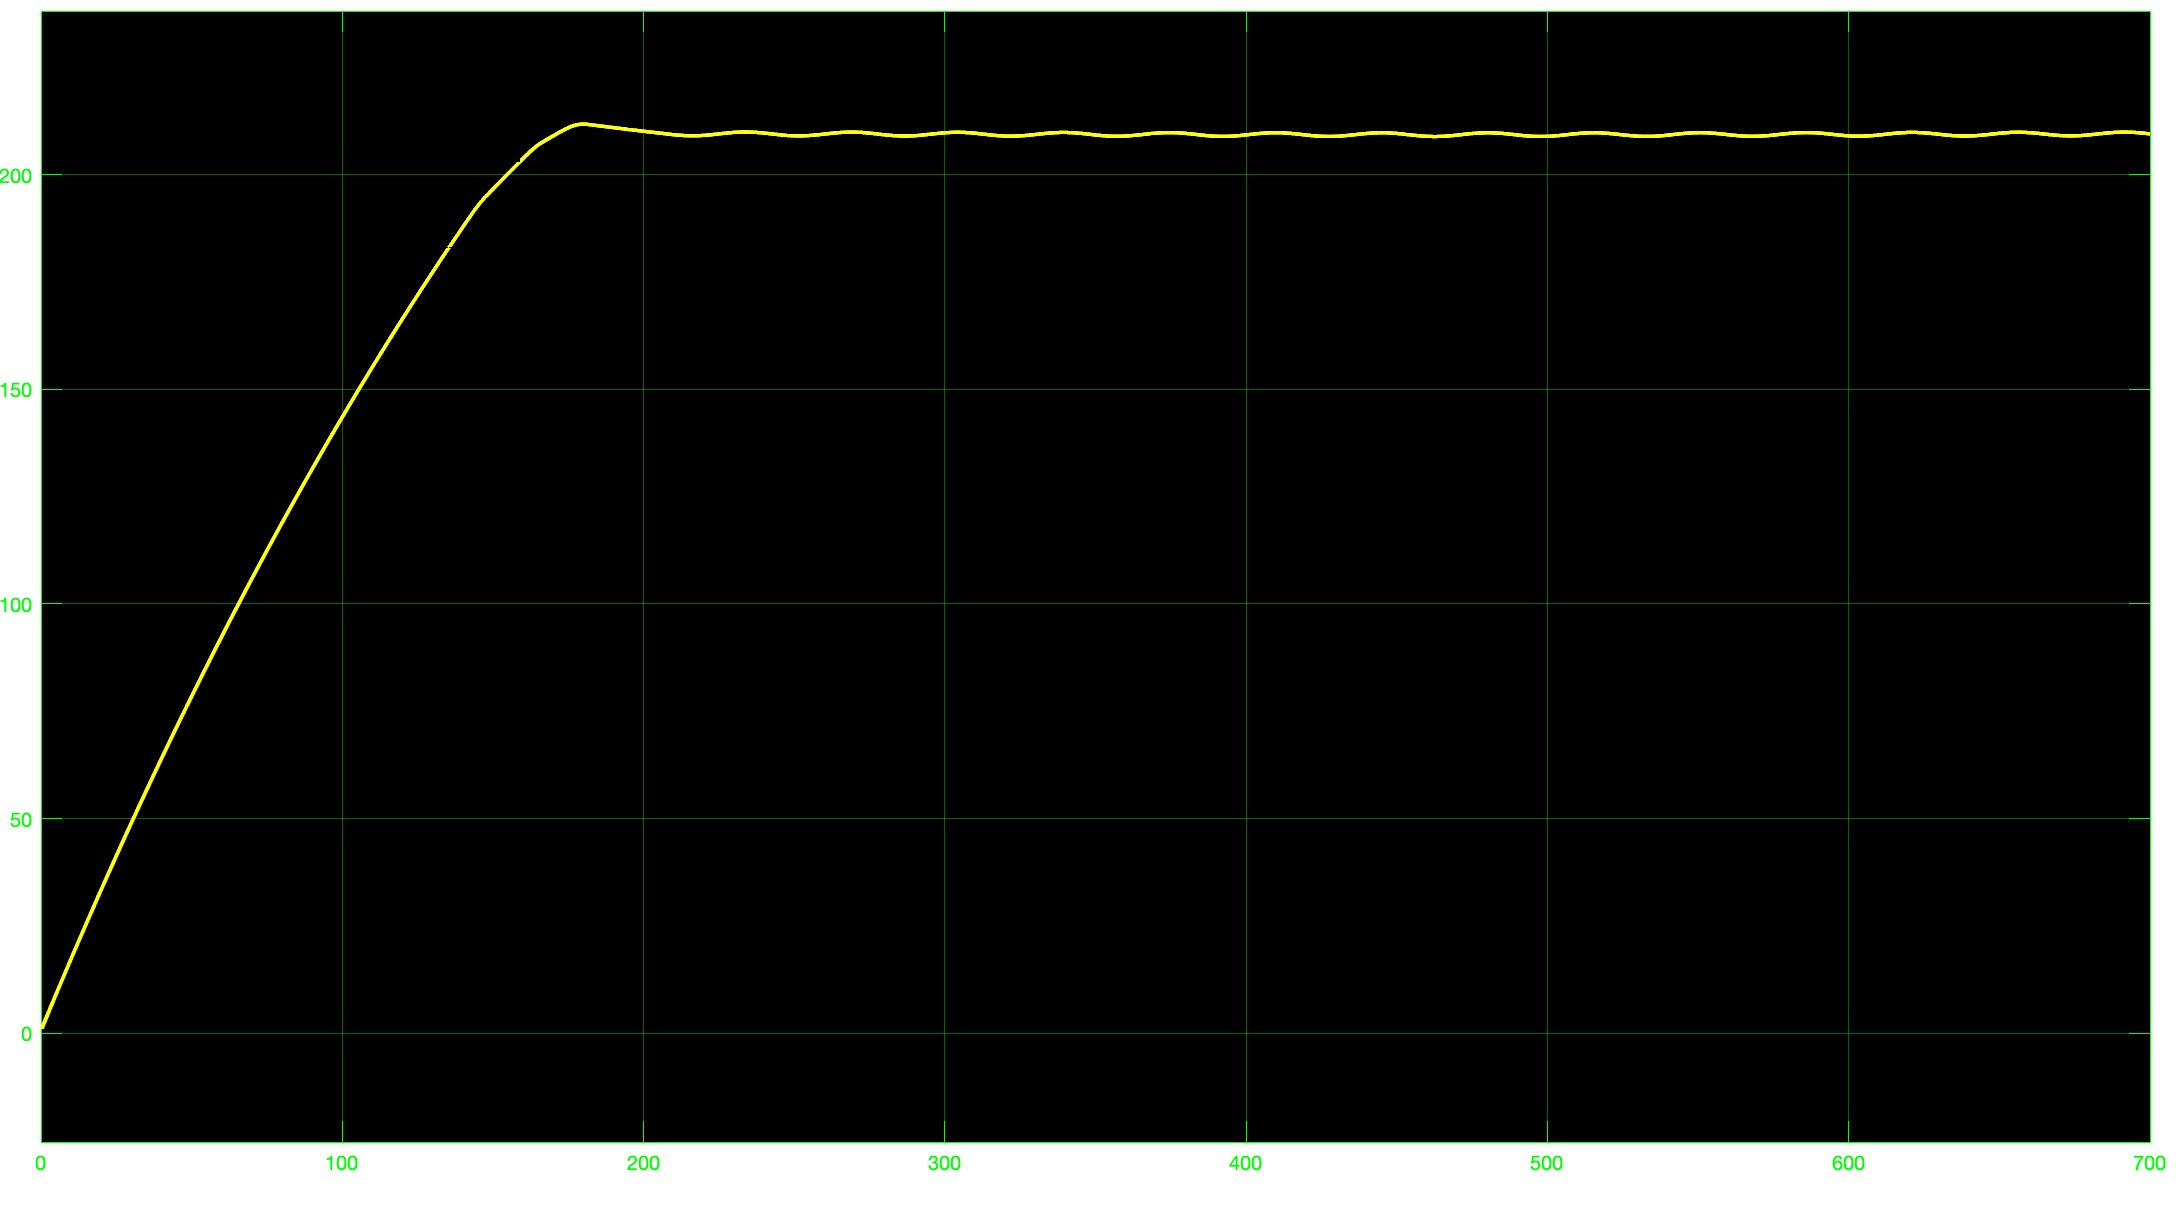
\includegraphics[scale=0.2]{punto_2/NonLin_x1e_x2e-1.jpg}
    \caption{$x_2$ = $x_{2e} - 1$}
    \label{fig:enter-label}
\end{figure}

\begin{figure}[!h]
    \centering
    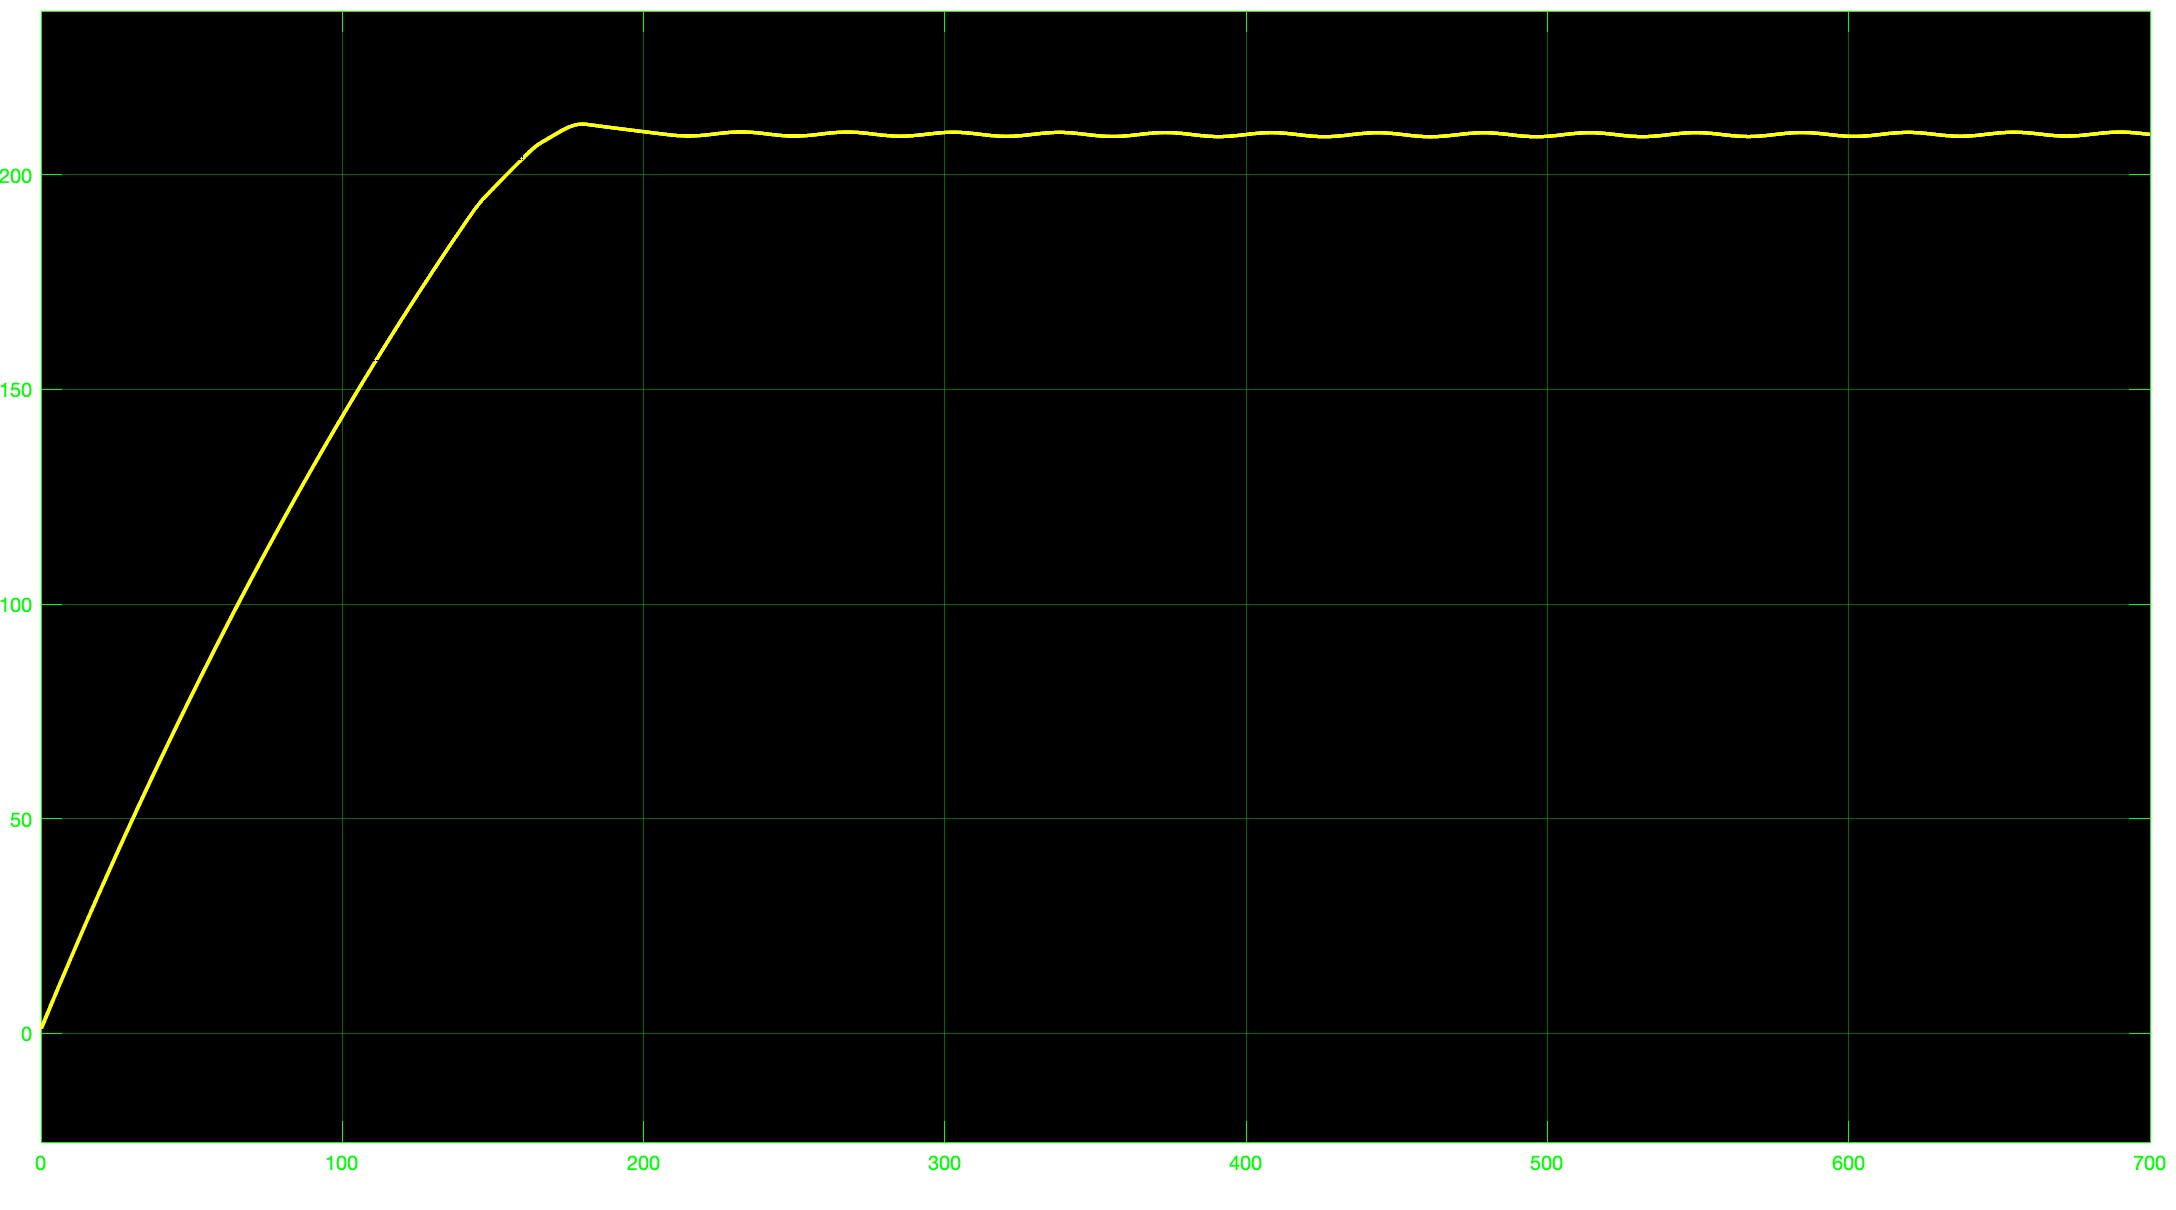
\includegraphics[scale=0.2]{punto_2/NonLin_x1e_x2e+1.jpg}
    \caption{$x_2$ = $x_{2e} + 1$}
    \label{fig:enter-label}
\end{figure}

\begin{figure}[!h]
    \centering
    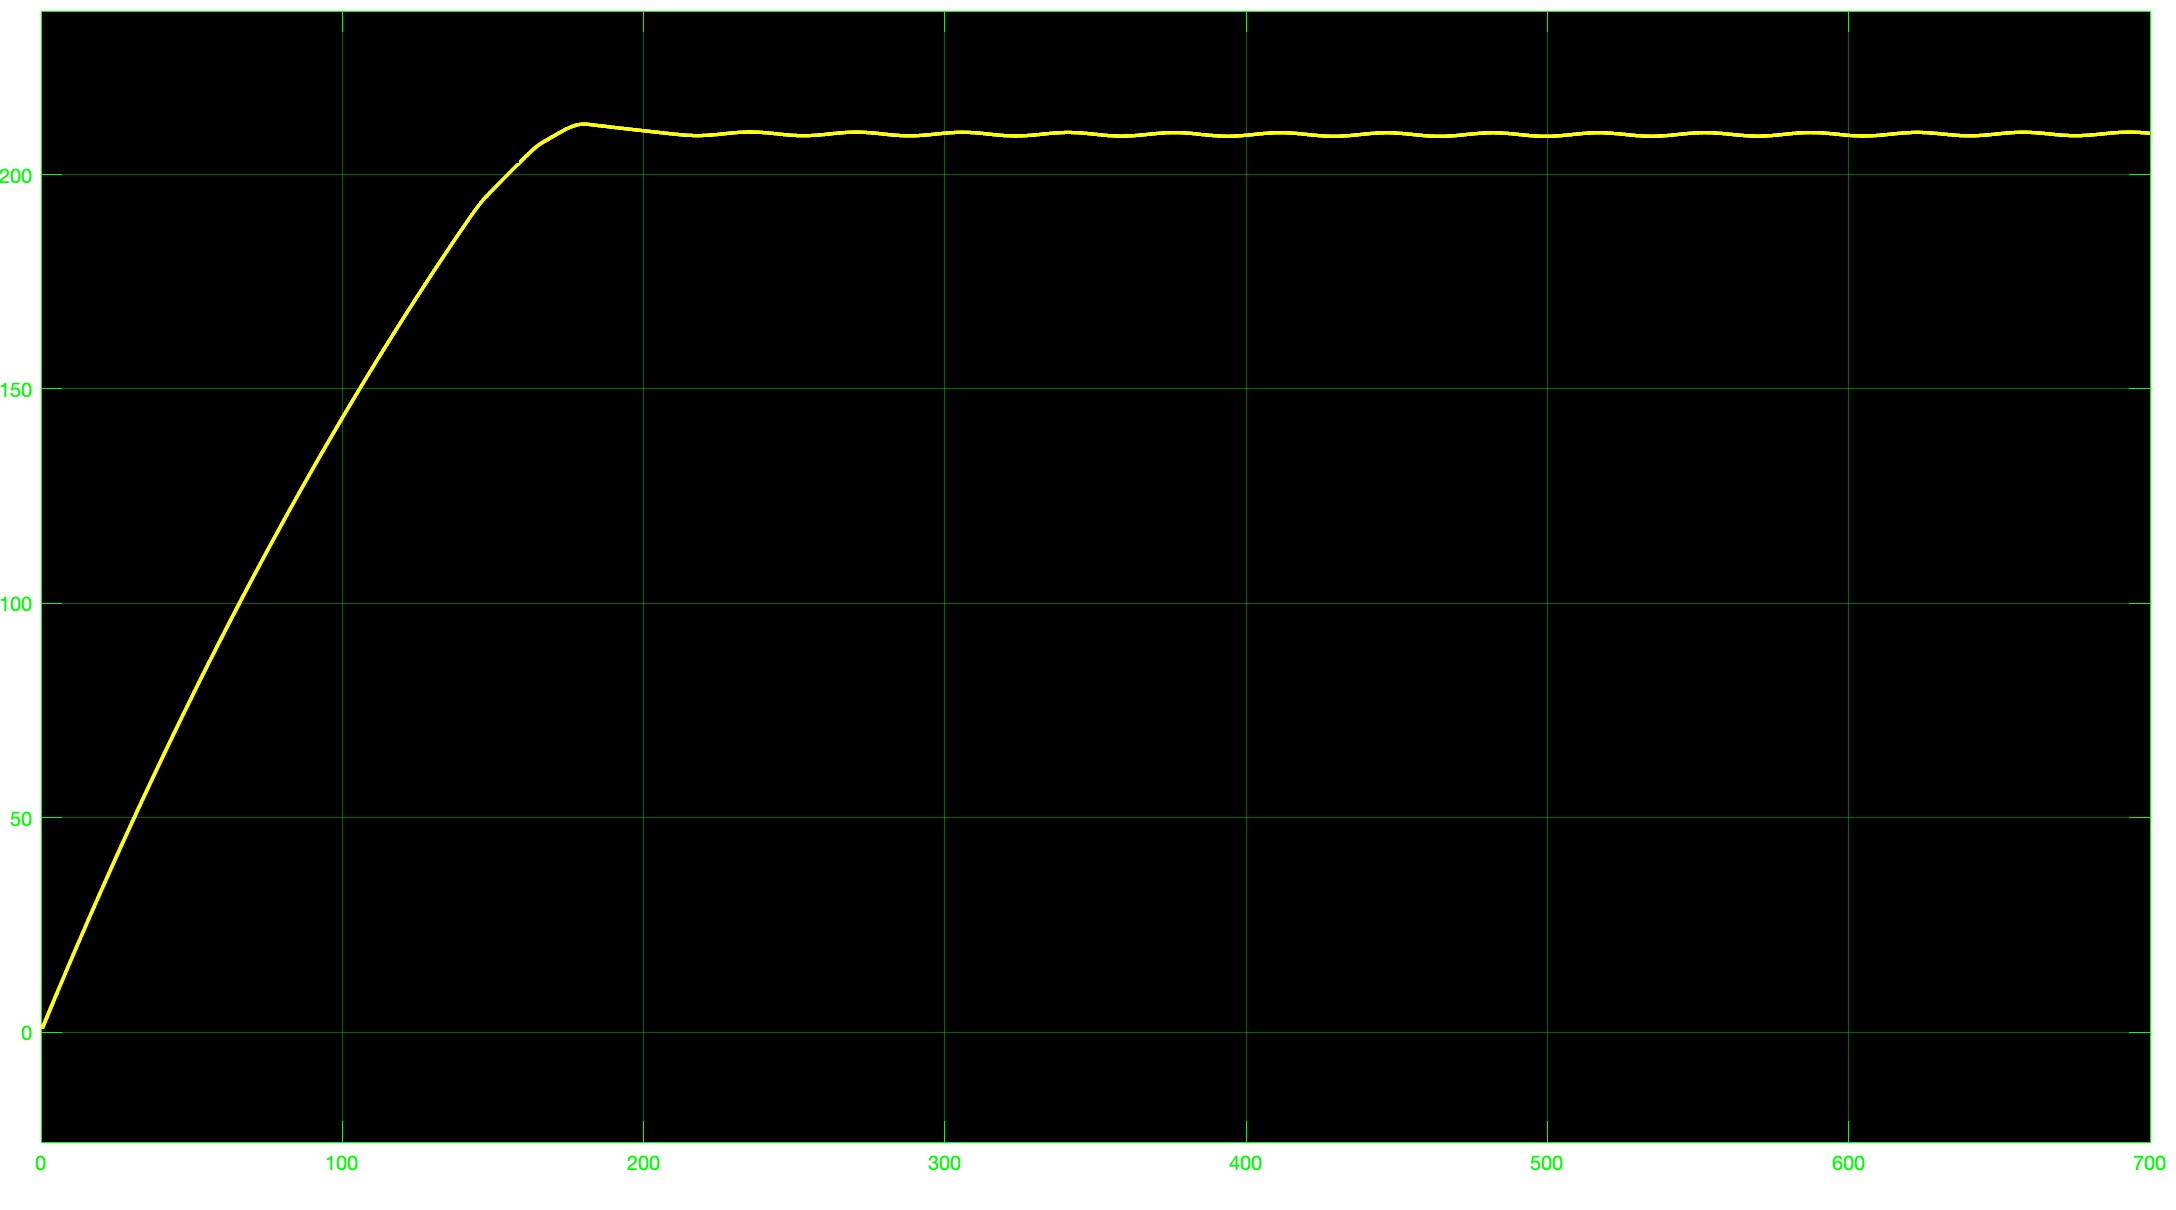
\includegraphics[scale=0.2]{punto_2/x2-3.jpg}
    \caption{$x_2$ = $x_{2e} - 3$}
    \label{fig:enter-label}
\end{figure}

\begin{figure}[!h]
    \centering
    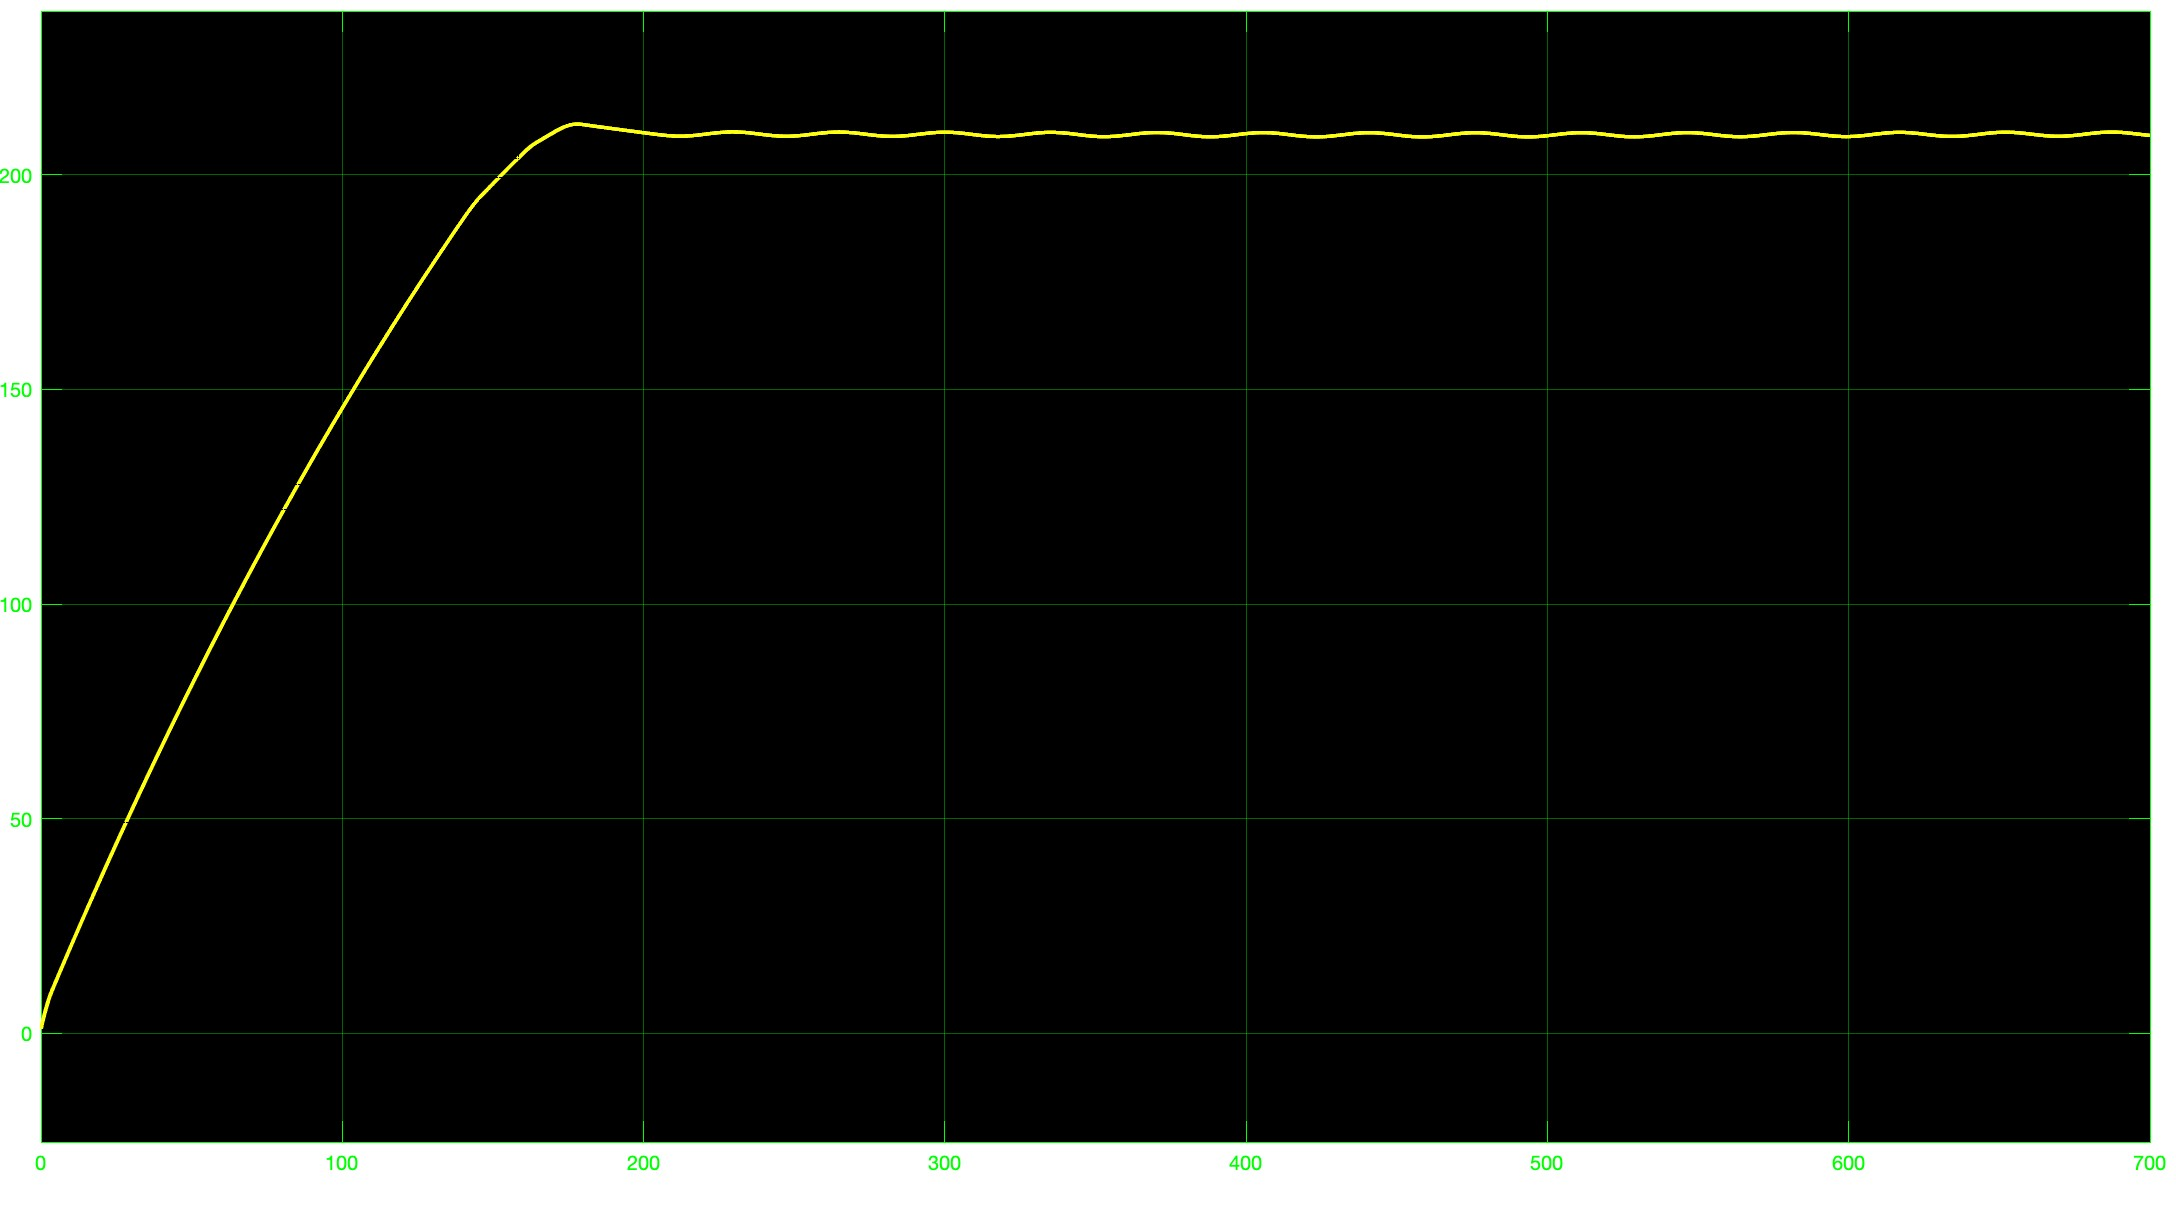
\includegraphics[scale=0.2]{punto_2/x2+3.jpg}
    \caption{$x_2$ = $x_{2e} + 3$}
    \label{fig:enter-label}
\end{figure}

\begin{figure}[!h]
    \centering
    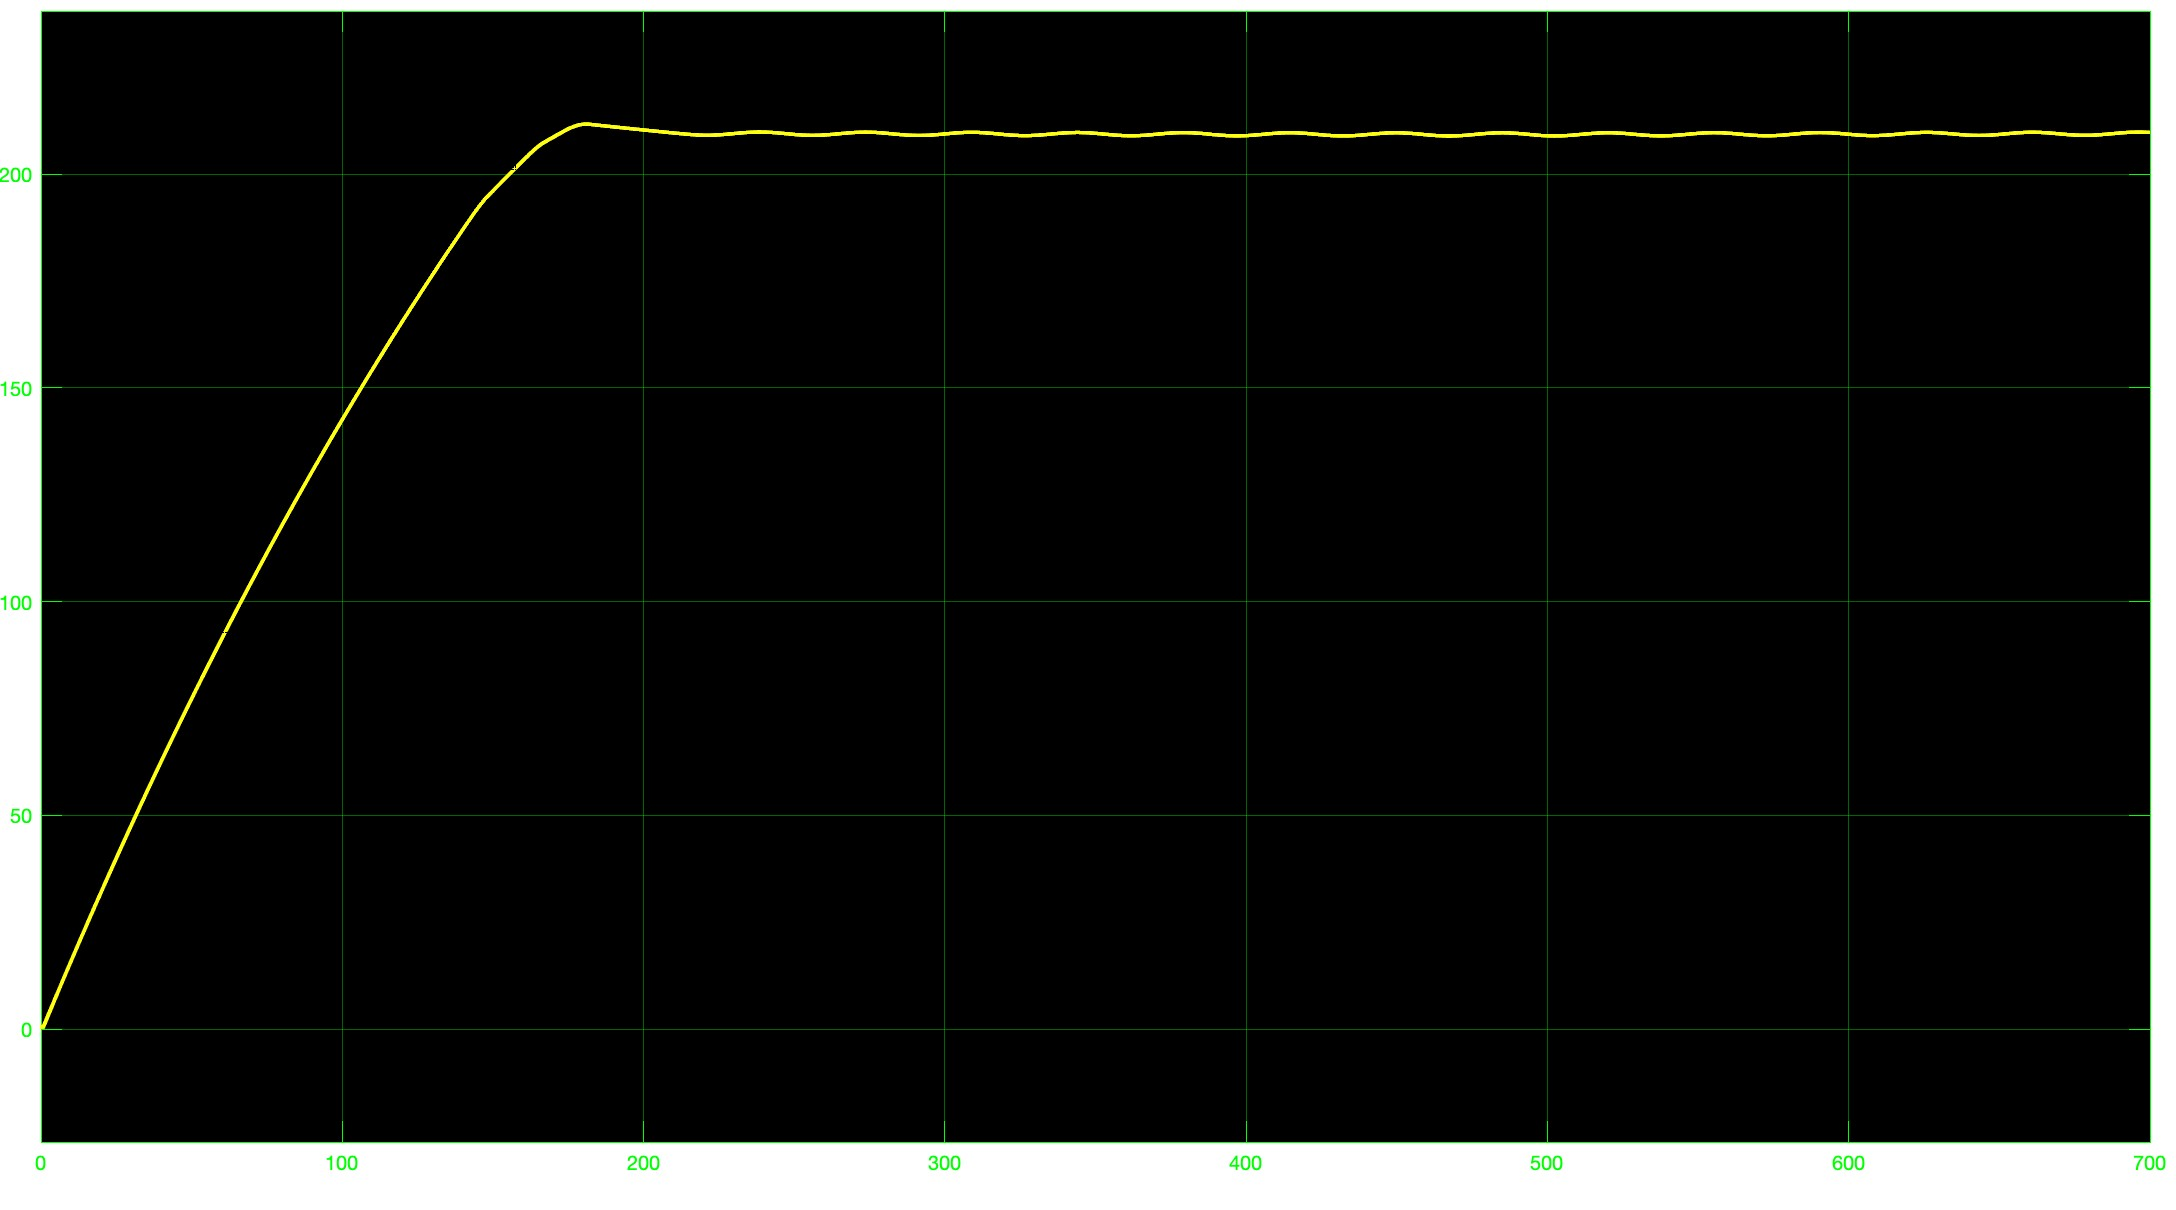
\includegraphics[scale=0.2]{punto_2/NonLin_x1e_x2e-6.jpg}
    \caption{$x_2$ = $x_{2e} - 6$}
    \label{fig:enter-label}
\end{figure}

\begin{figure}[!h]
    \centering
    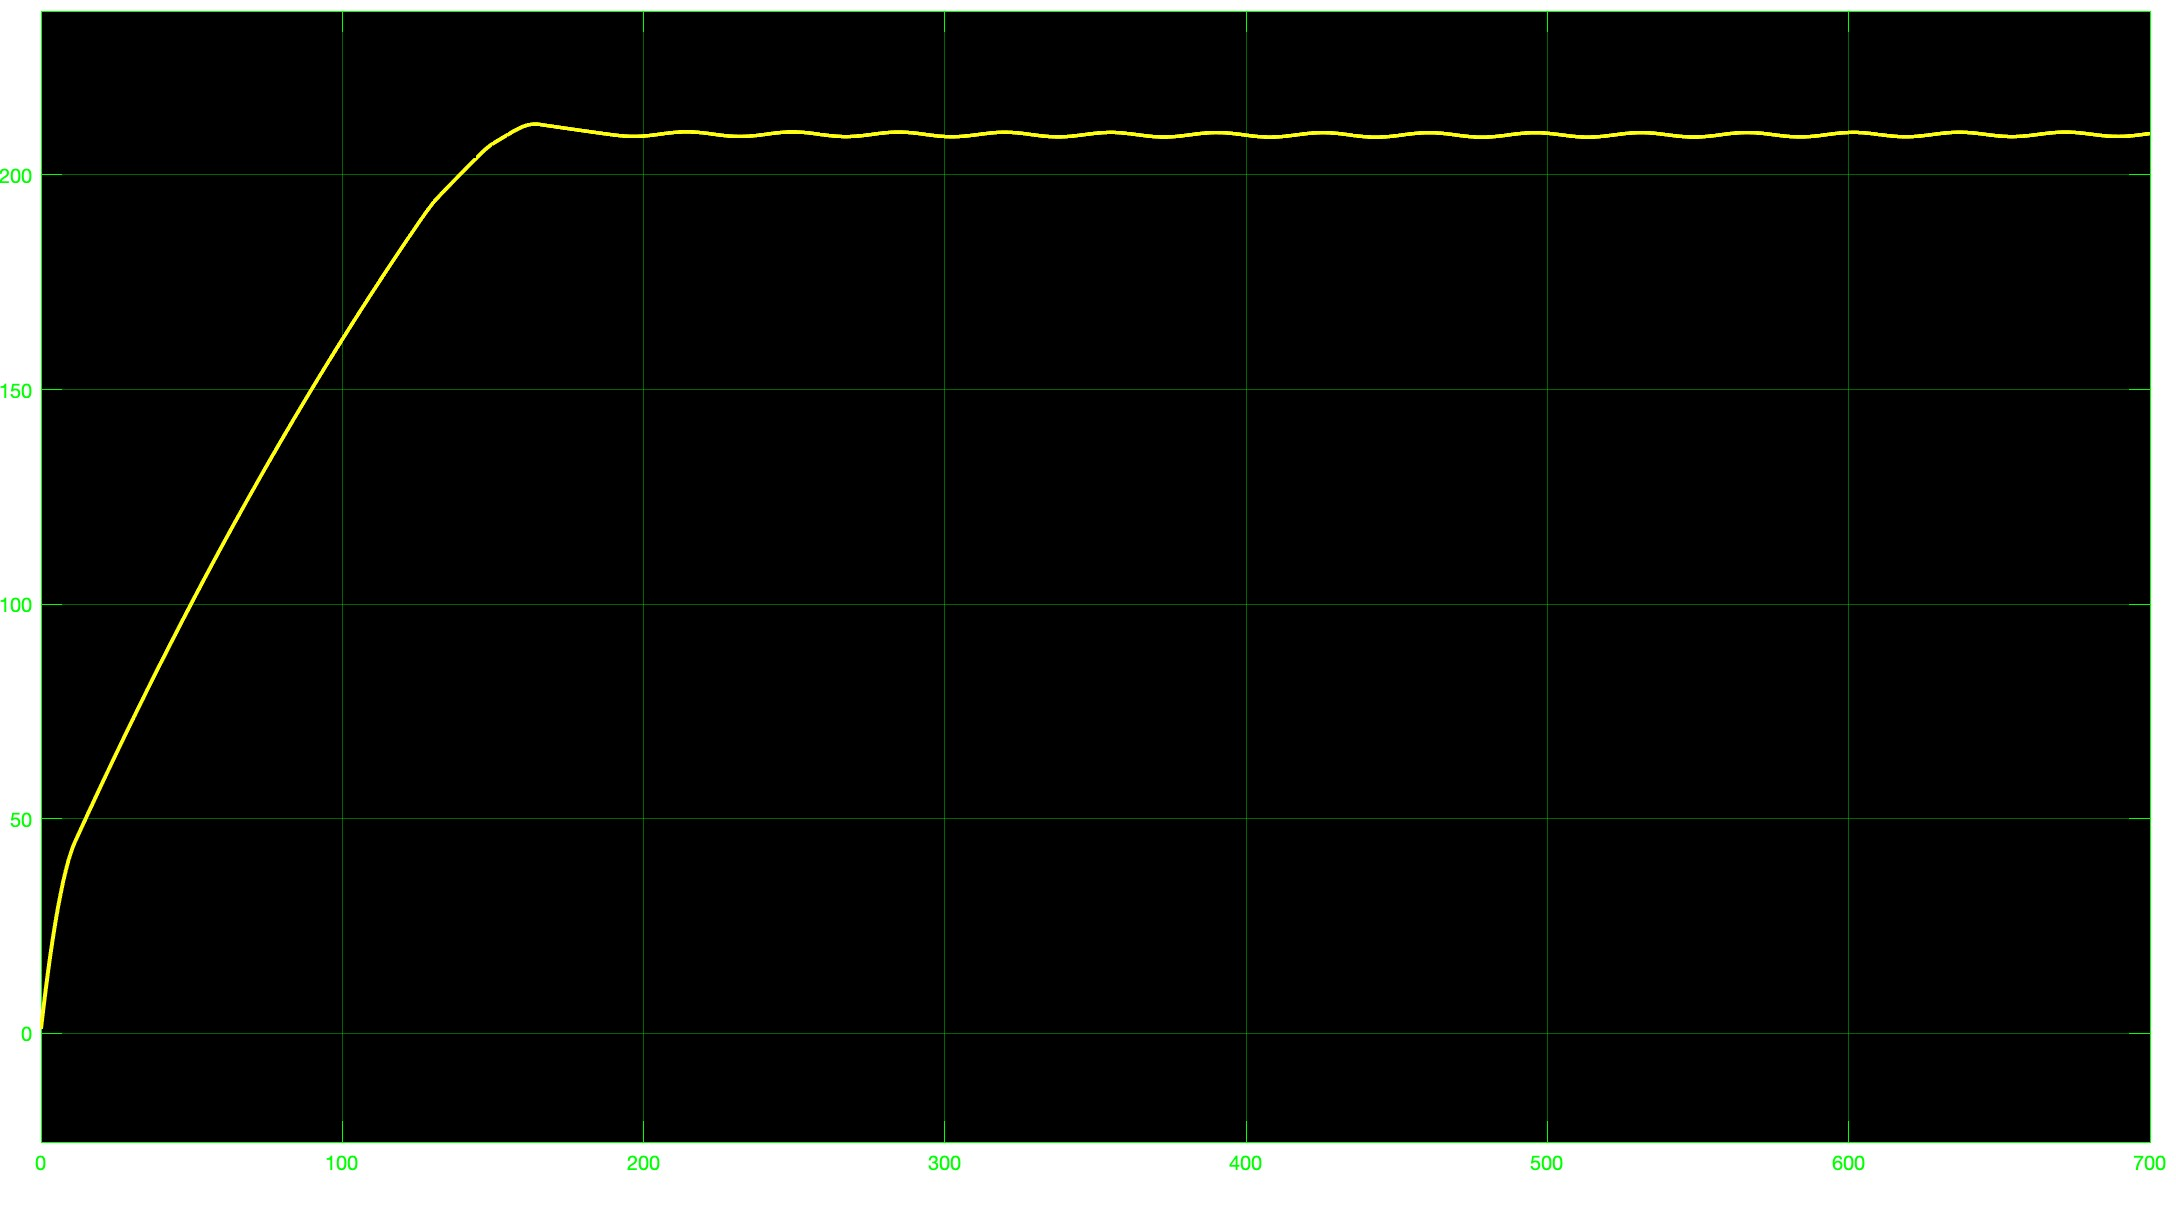
\includegraphics[scale=0.2]{punto_2/x2e+6.jpg}
    \caption{$x_2$ = $x_{2e} - 6$}
    \label{fig:enter-label}
\end{figure}

\begin{figure}[!h]
    \centering
    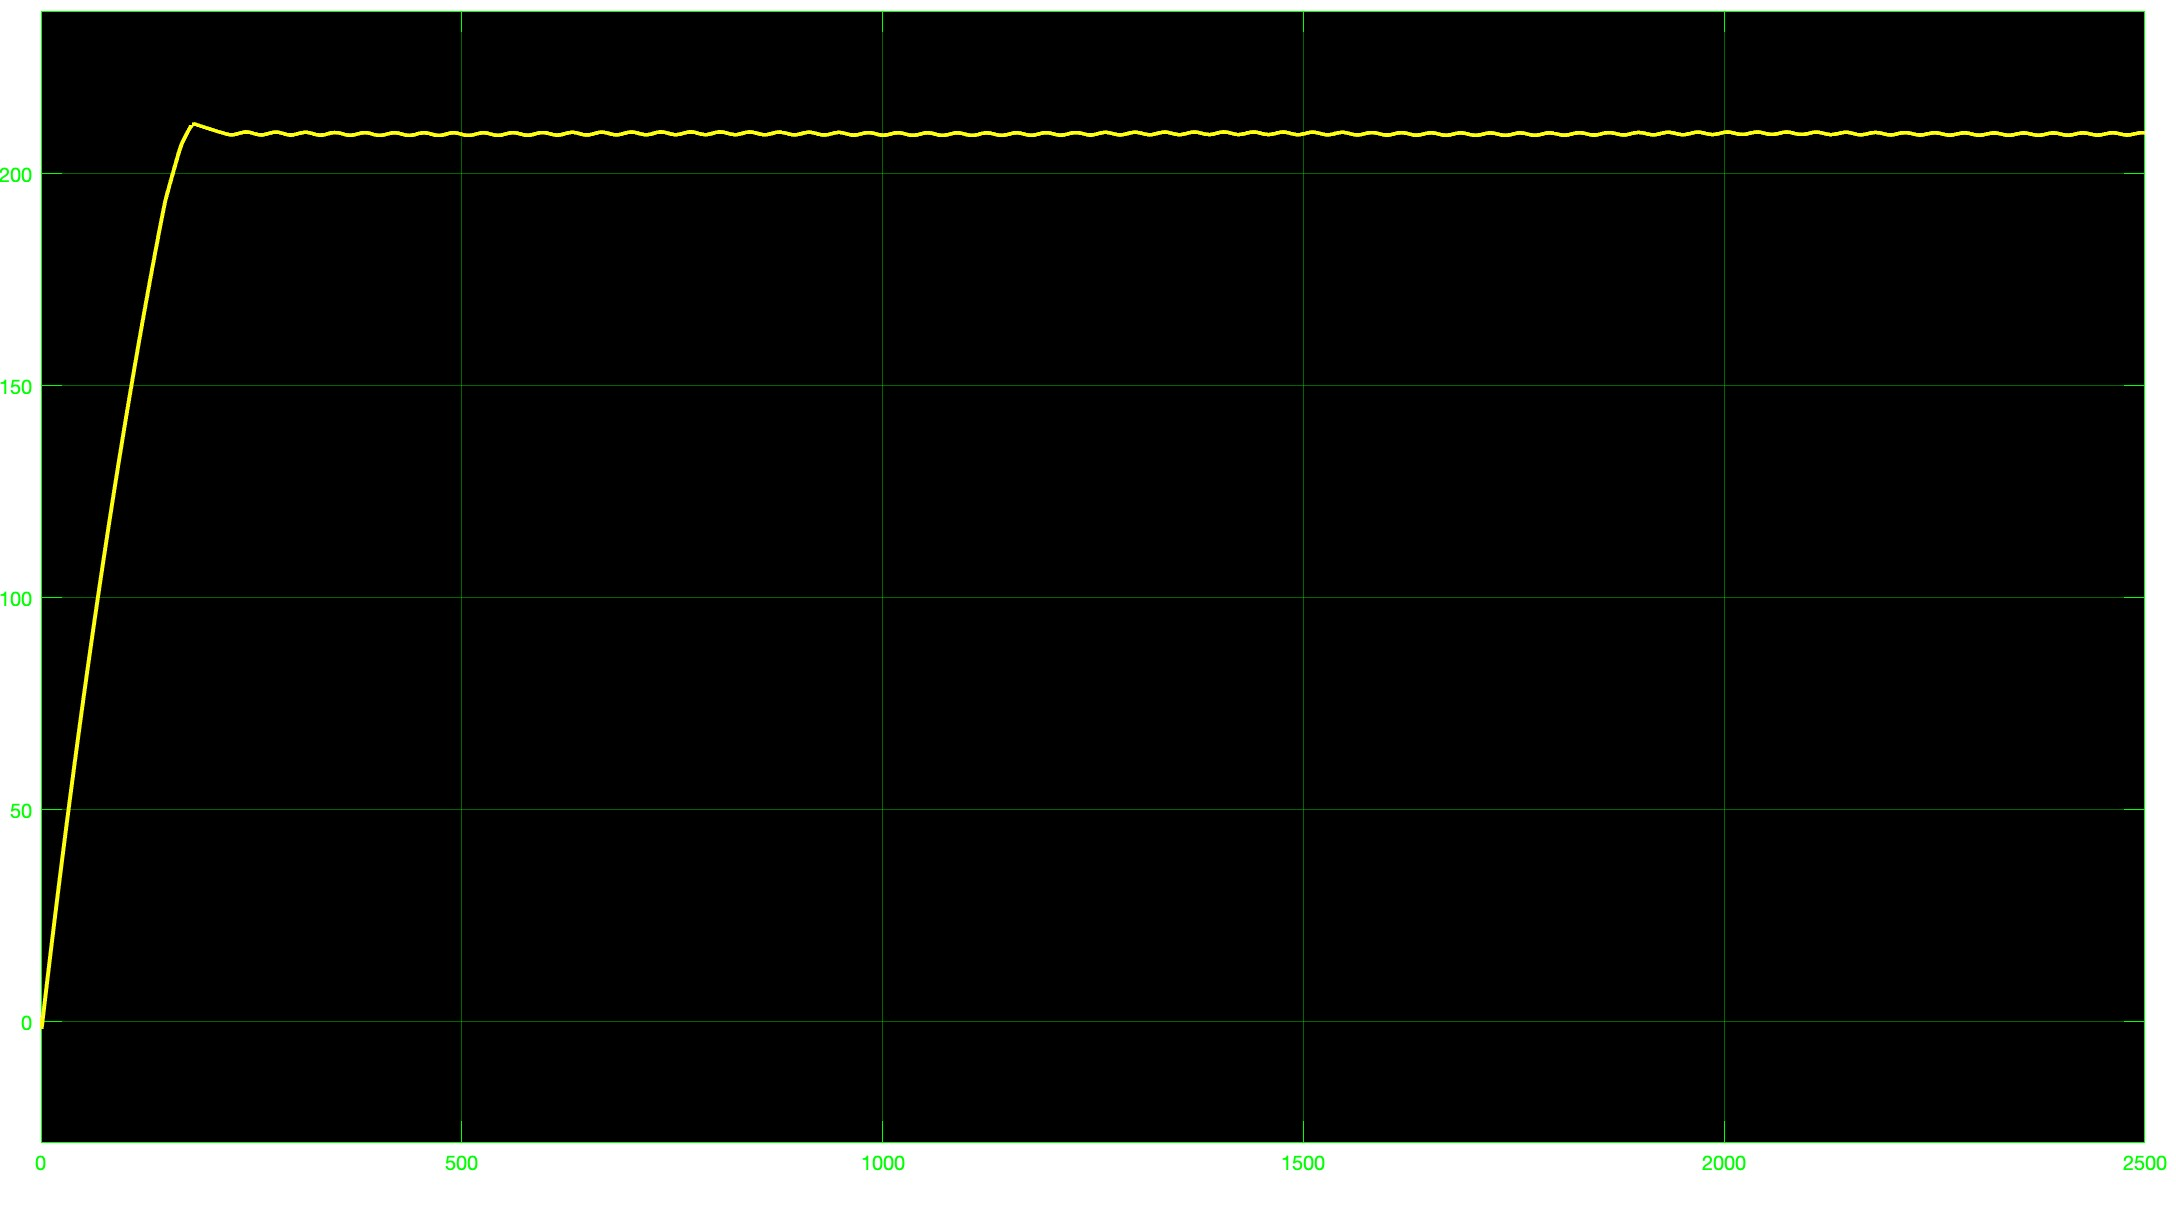
\includegraphics[scale=0.2]{punto_2/NoLin_x2e-10.jpg}
    \caption{$x_2$ = $x_{2e} - 10$}
    \label{fig:enter-label}
\end{figure}

\begin{figure}[!h]
    \centering
    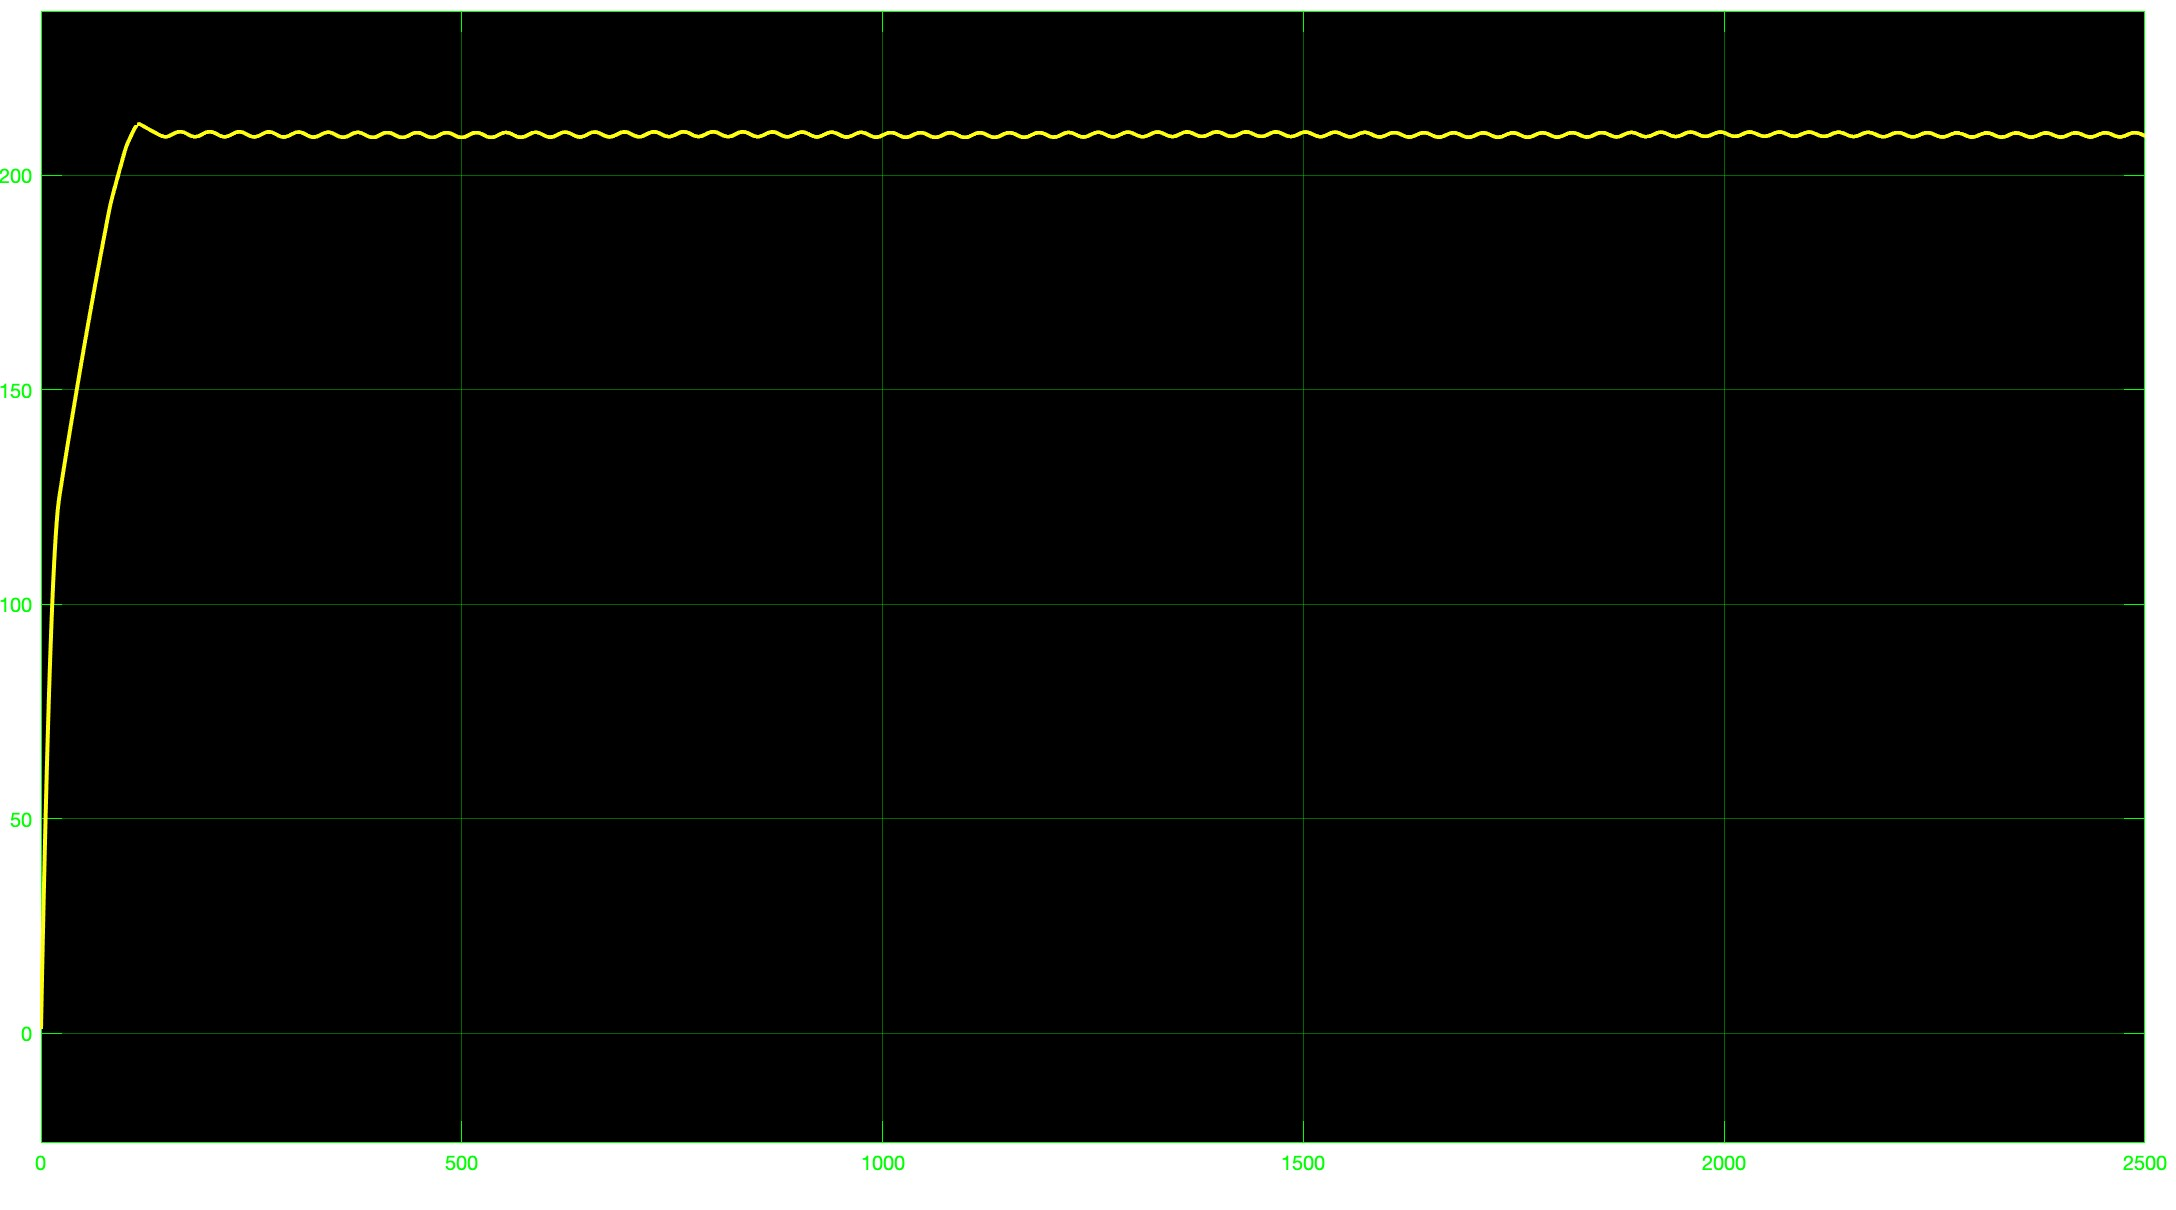
\includegraphics[scale=0.2]{punto_2/NoLin_x2e+10.jpg}
    \caption{$x_2$ = $x_{2e} + 10$}
    \label{fig:enter-label}
\end{figure}

\begin{figure}[!h]
    \centering
    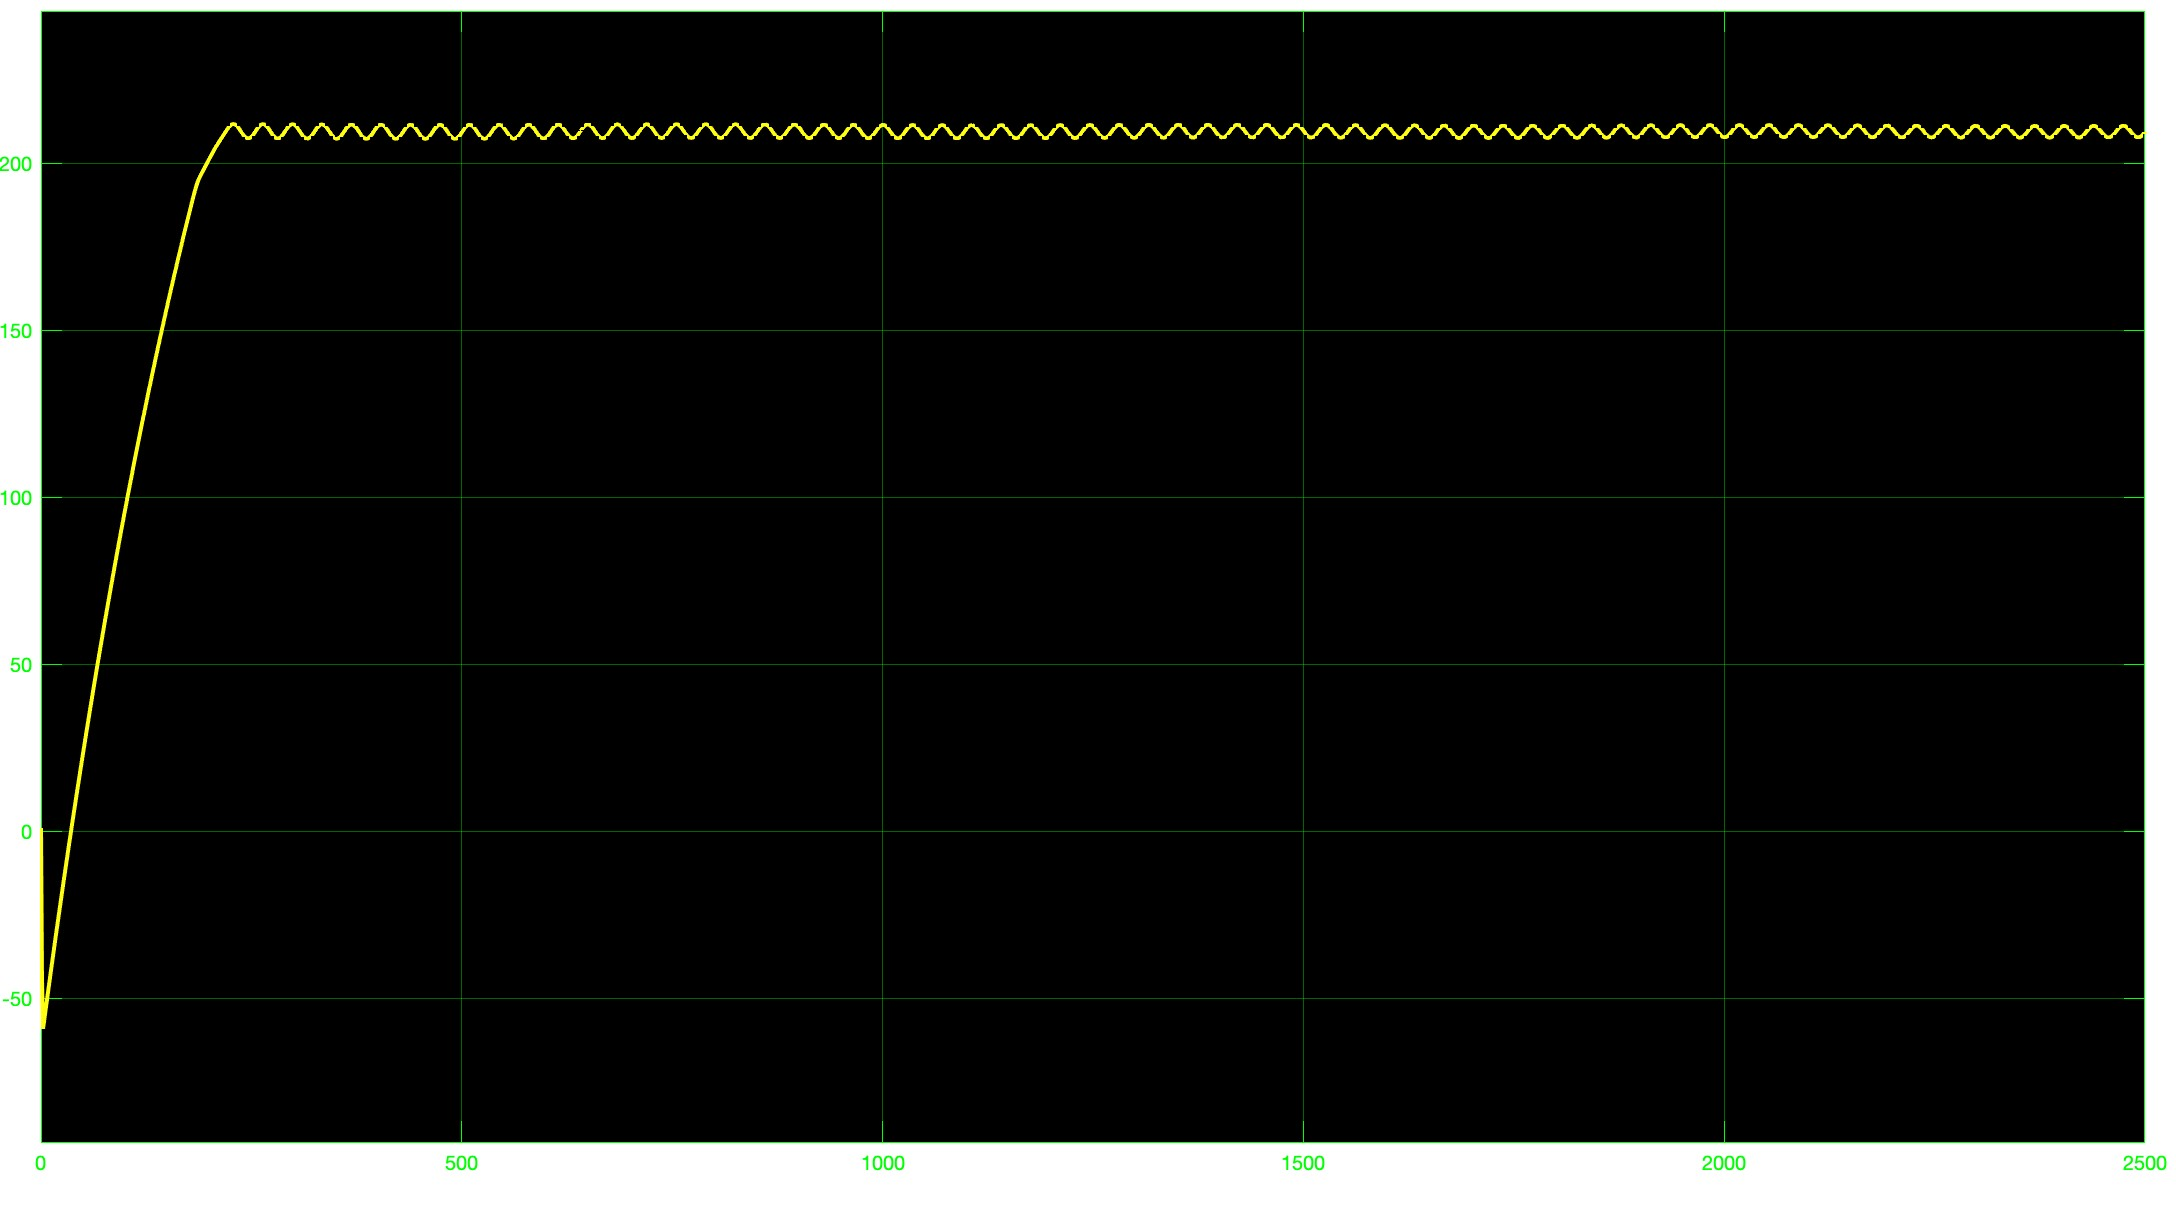
\includegraphics[scale=0.2]{punto_2/NoLin_x2e-50.jpg}
    \caption{$x_2$ = $x_{2e} - 50$}
    \label{fig:enter-label}
\end{figure}

\vspace{0.5cm}

\begin{figure}[!h]
    \centering
    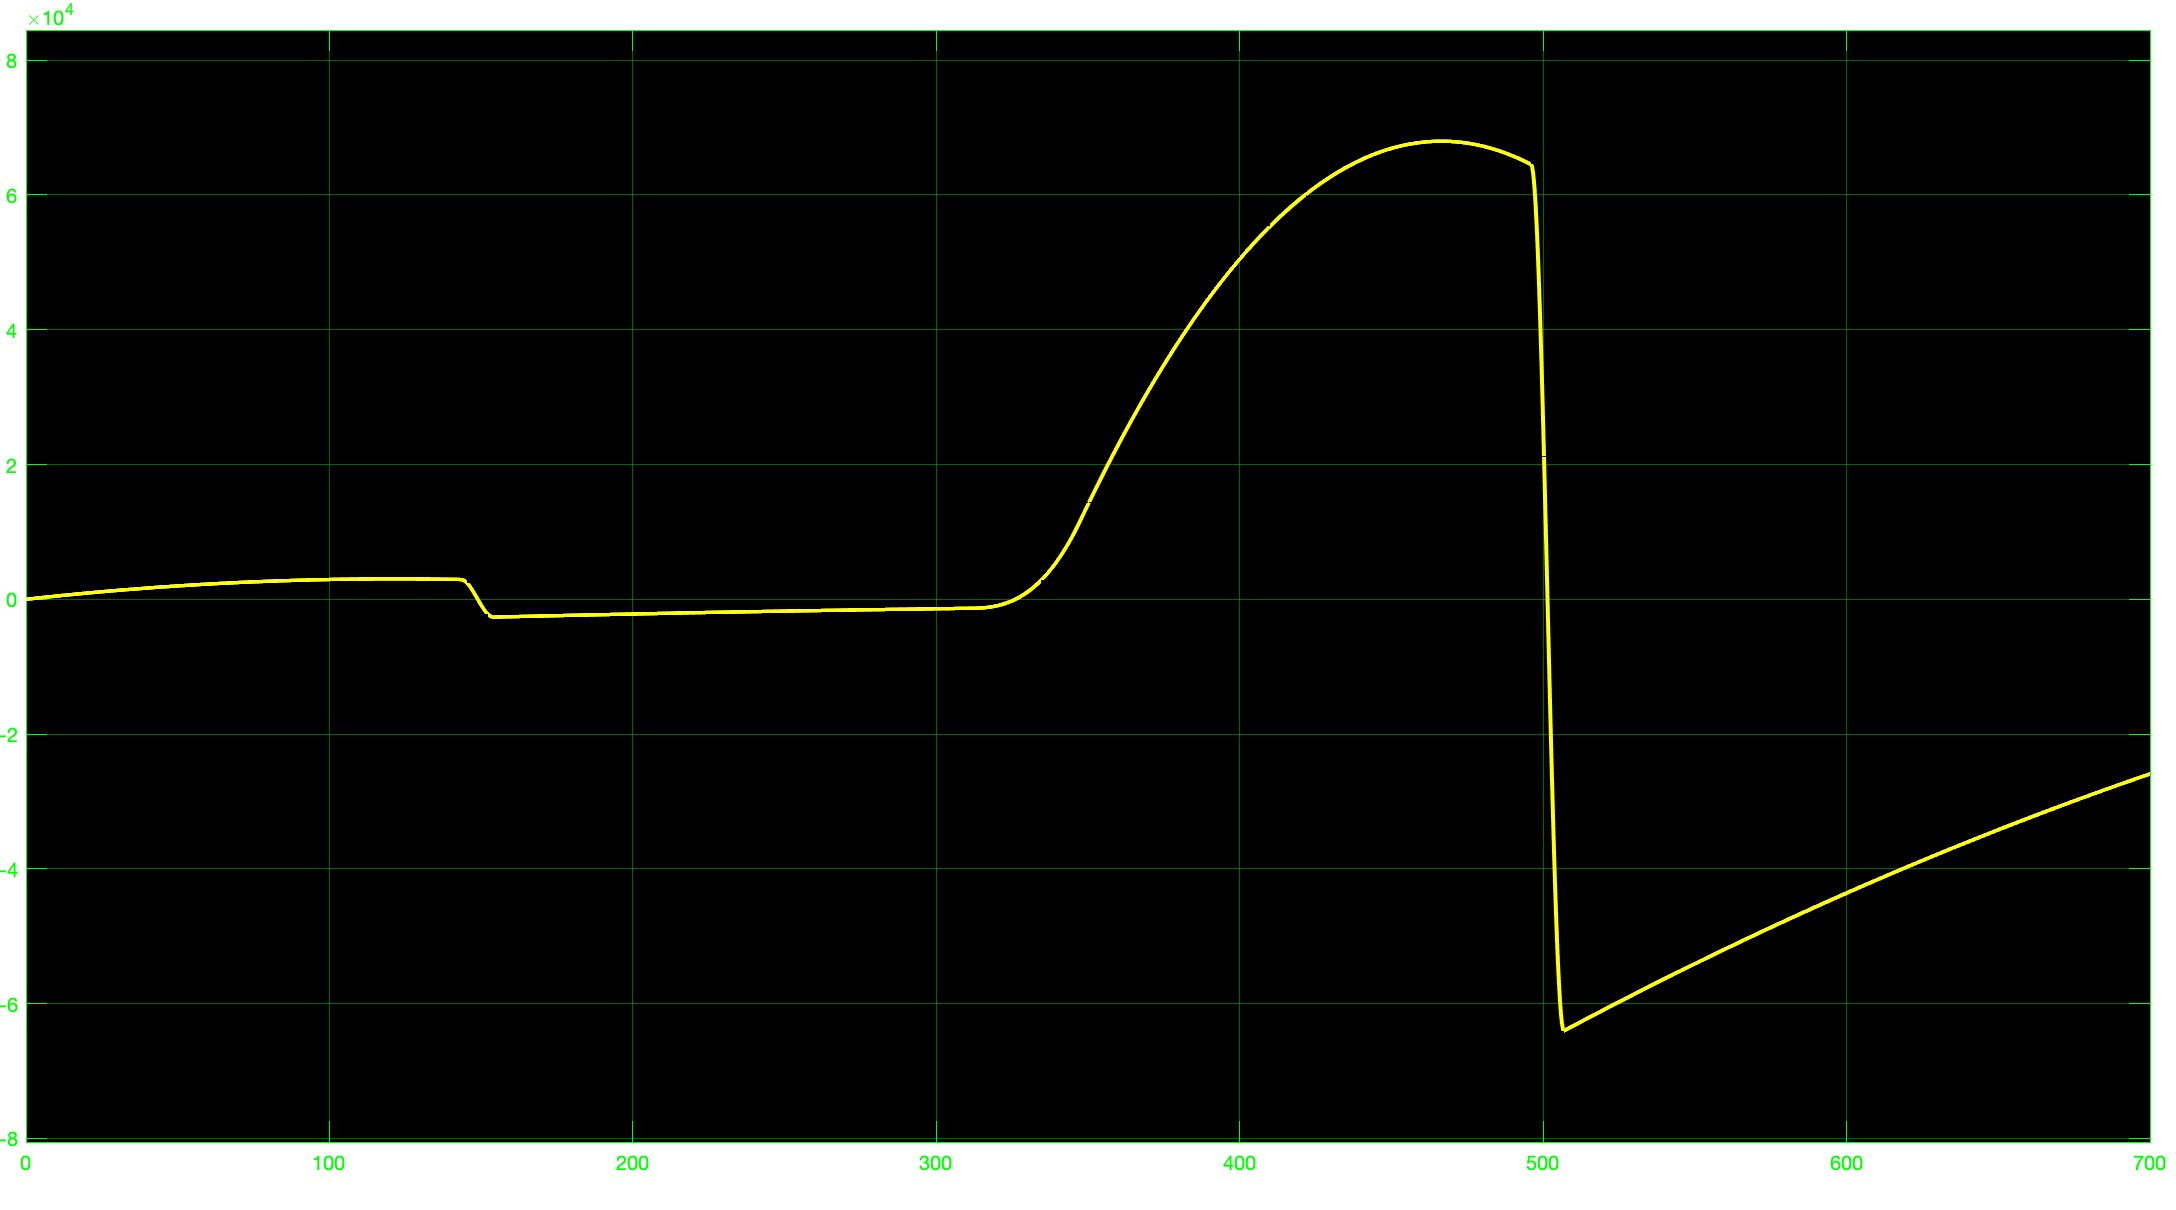
\includegraphics[scale=0.2]{punto_2/x2+50.jpg}
    \caption{$x_2$ = $x_{2e} + 50$}
    \label{fig:enter-label}
\end{figure}

\clearpage

Per valori compresi tra -50 e +10, dopo un certo intervallo di tempo si stabilizza, come si nota in Figura 16-23. Diversamente, per valori molto superiori di 10 (Figura 24), il sistema tende ad essere instabile.

\subsection{Terzo punto}
Un aspetto fondamentale è la valutazione della robustezza del controllore rispetto alle variazioni dell'ampiezza dei riferimenti a gradino, poiché tali variazioni possono influire significativamente sul comportamento del sistema. Nel corso di questa analisi, ci proponiamo di esplorare il range di ampiezze di riferimenti a gradino per i quali il controllore mantiene un controllo efficace sul sistema non lineare.

\begin{figure}[!h]
    \centering
    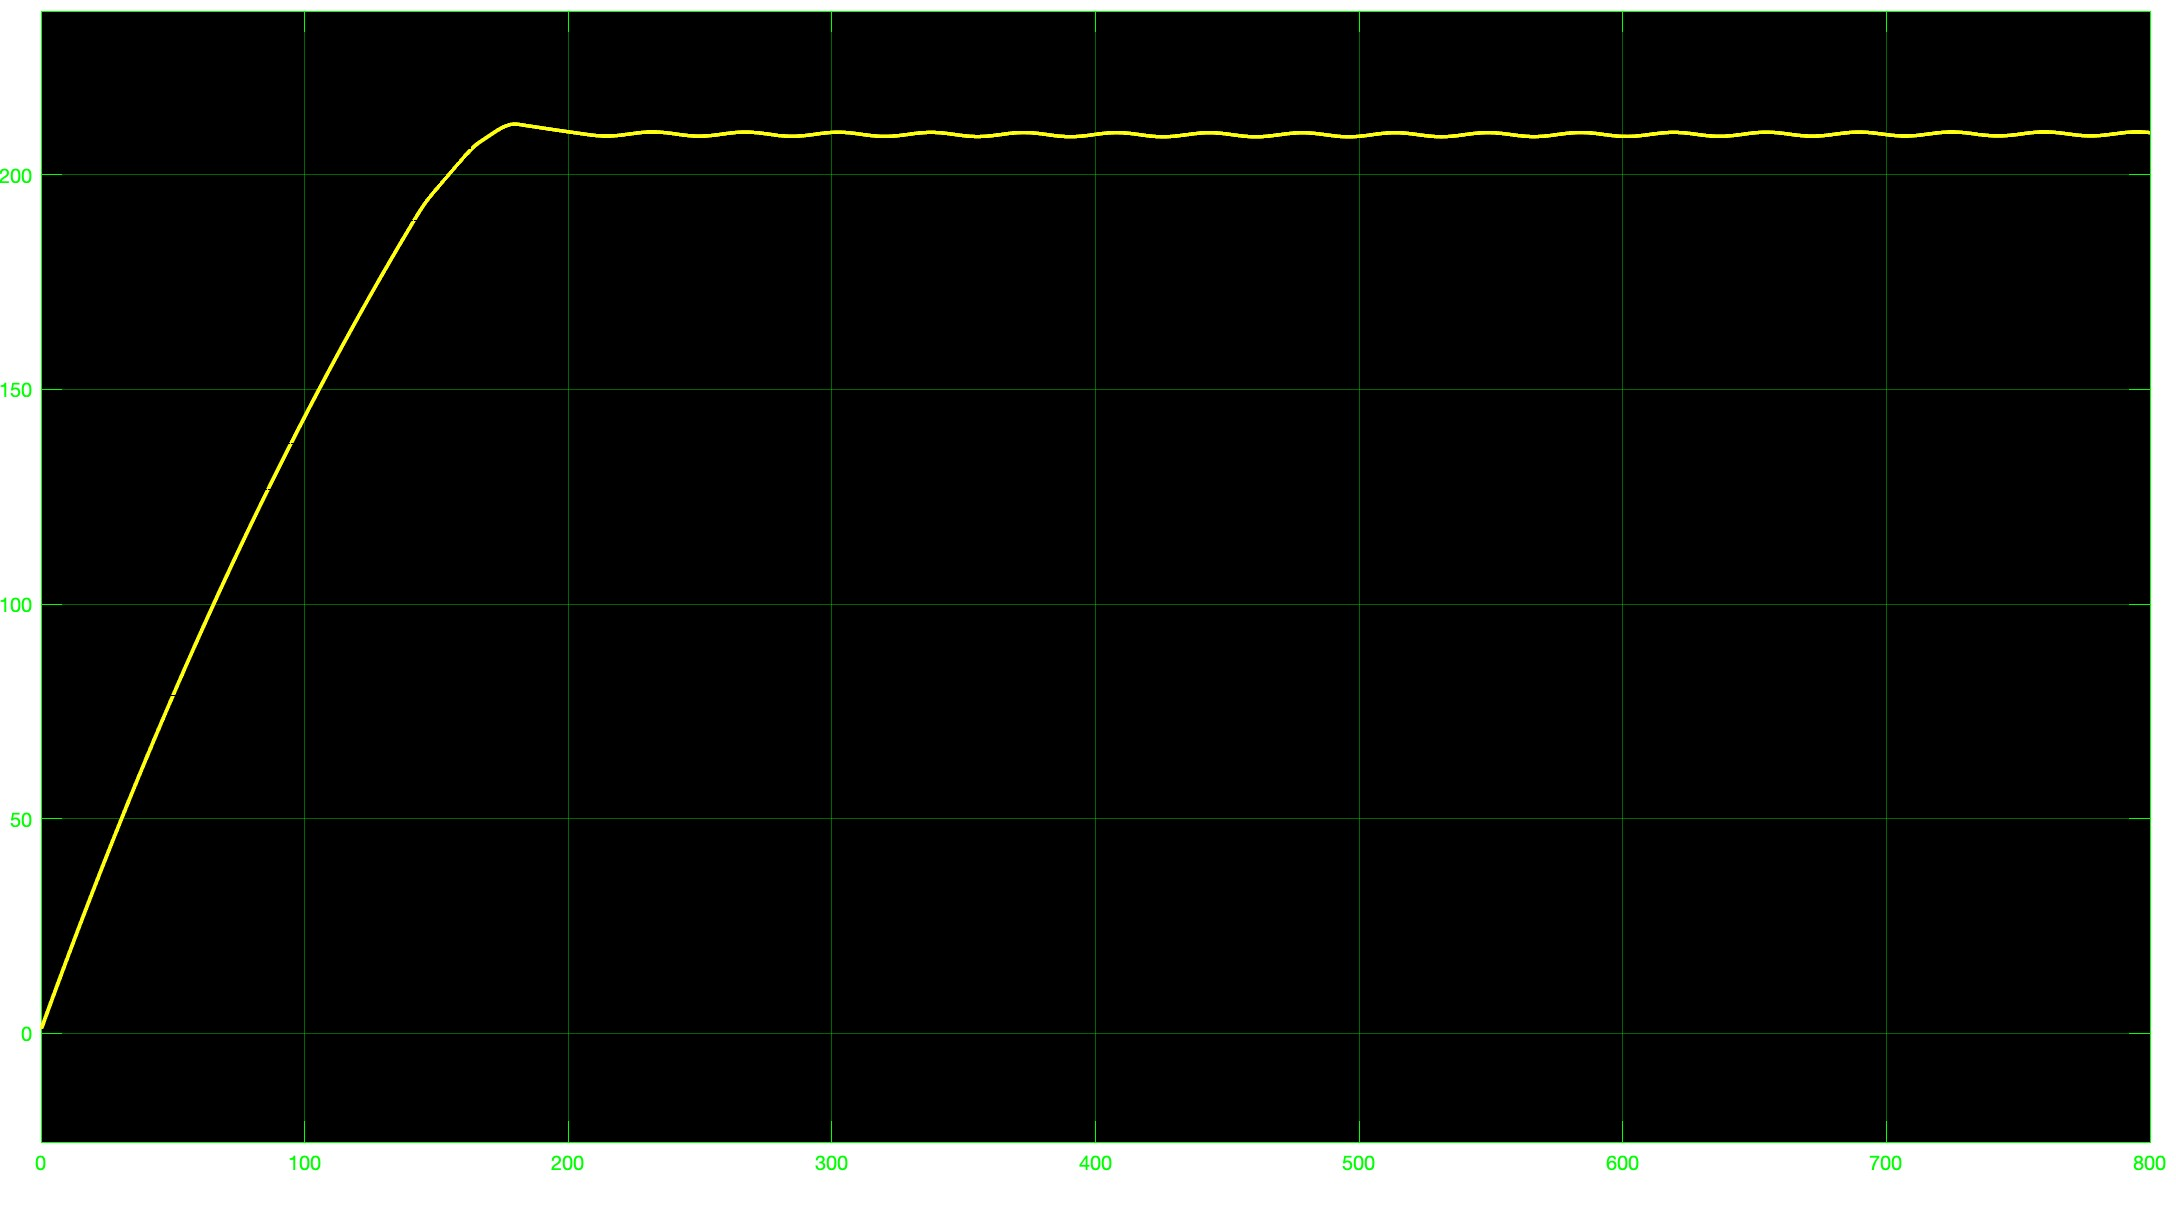
\includegraphics[scale=0.2]{Step_nonLineare/Step1_noLin.jpg}
    \caption{Risposta al gradino di ampiezza 1}
    \label{fig:enter-label}
\end{figure}

\begin{figure}[!h]
    \centering
    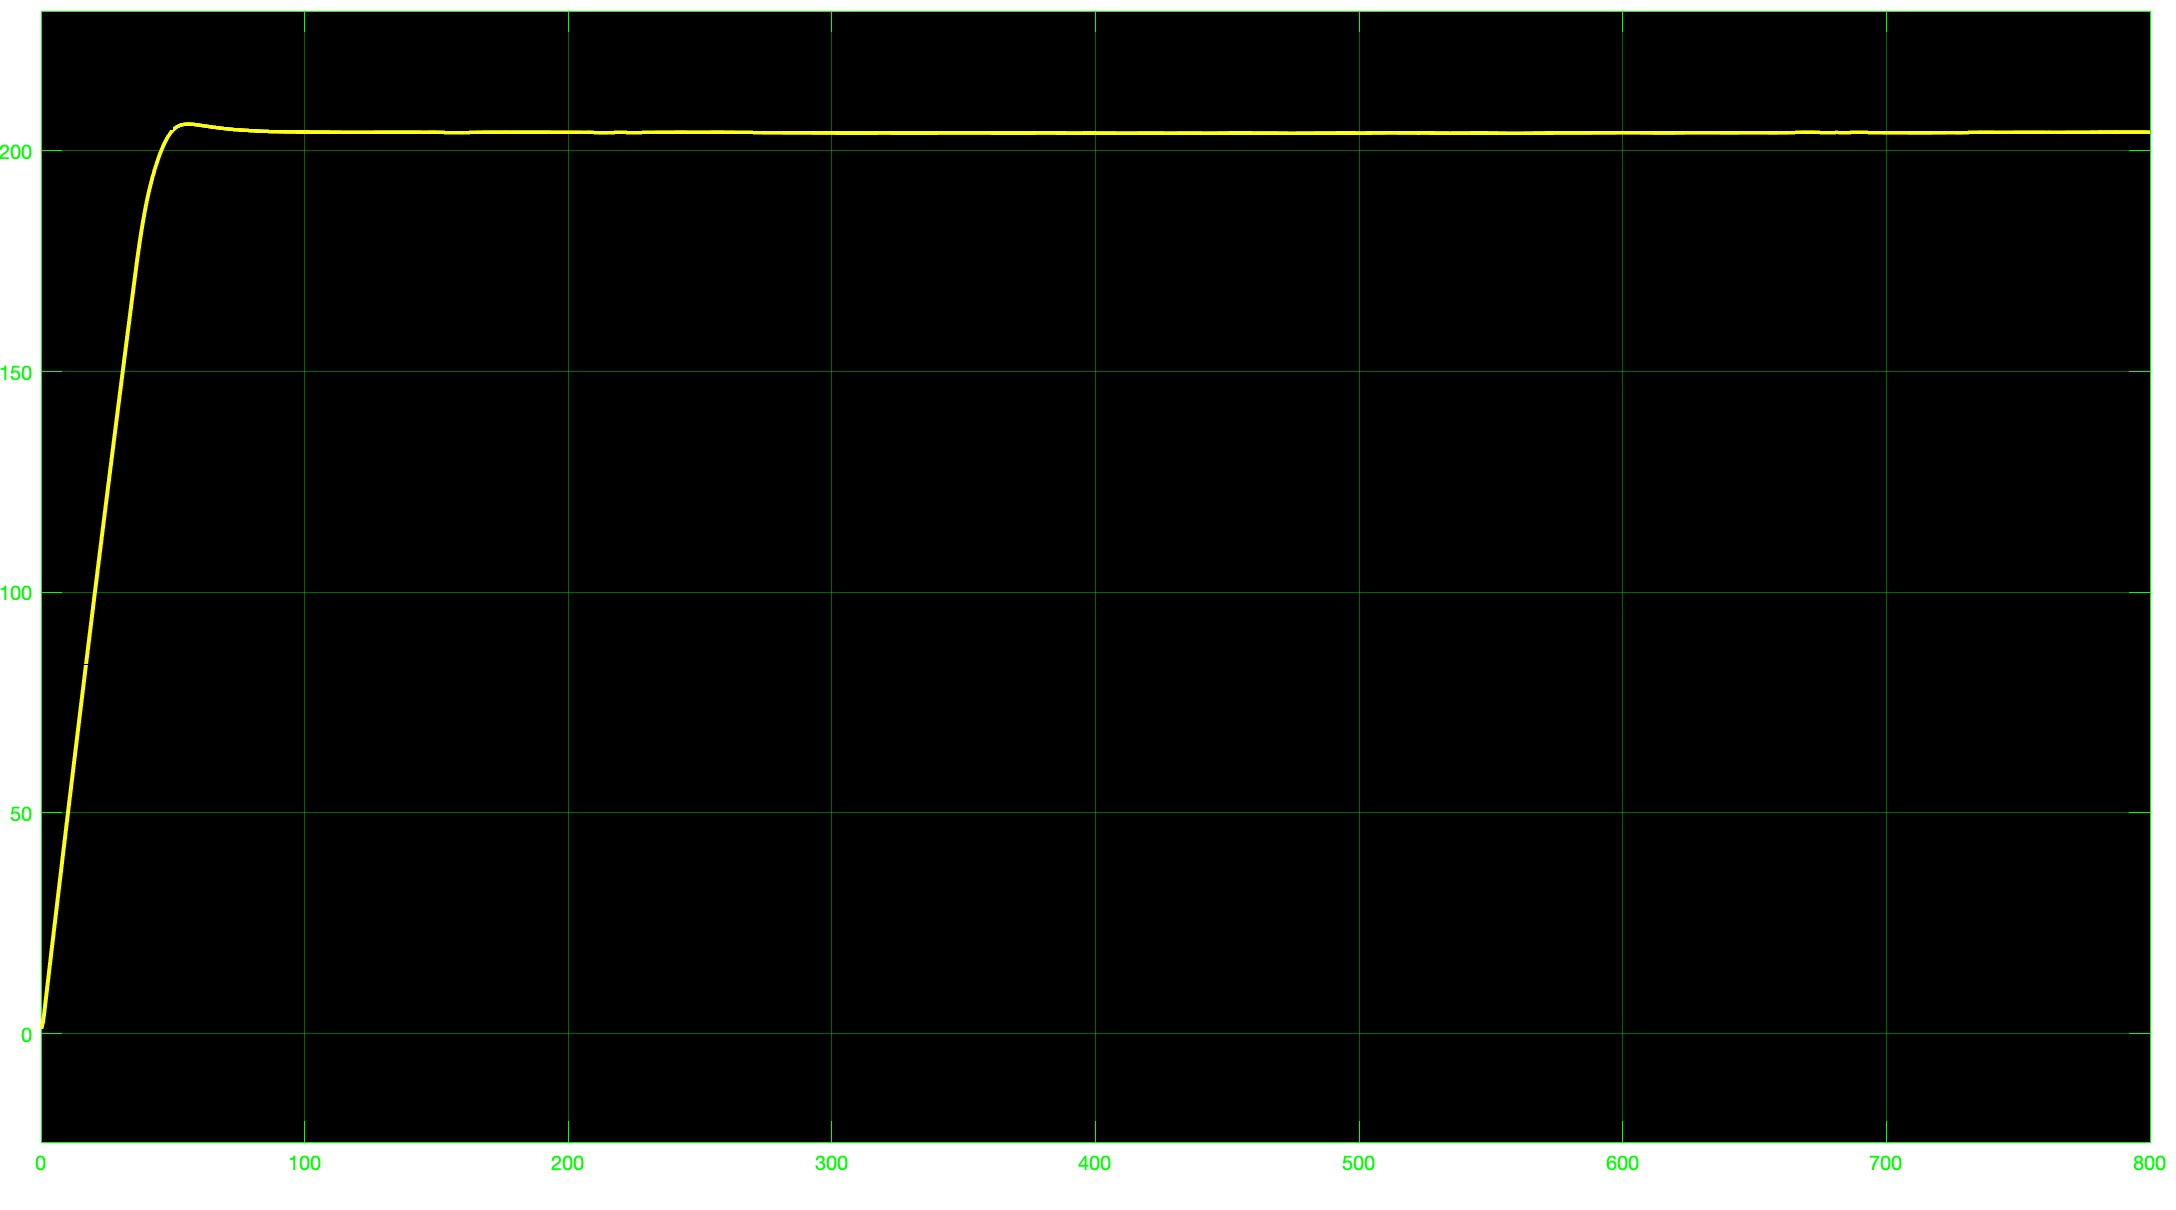
\includegraphics[scale=0.2]{Step_nonLineare/Step2_noLin.jpg}
    \caption{Risposta al gradino di ampiezza 2}
    \label{fig:enter-label}
\end{figure}

Nella Figura 25 e nella Figura 26, osserviamo che per valori di ampiezza inferiori o uguali a 2, il sistema non lineare presenta un comportamento simile alla risposta al gradino del sistema linearizzato.

\begin{figure}[!h]
    \centering
    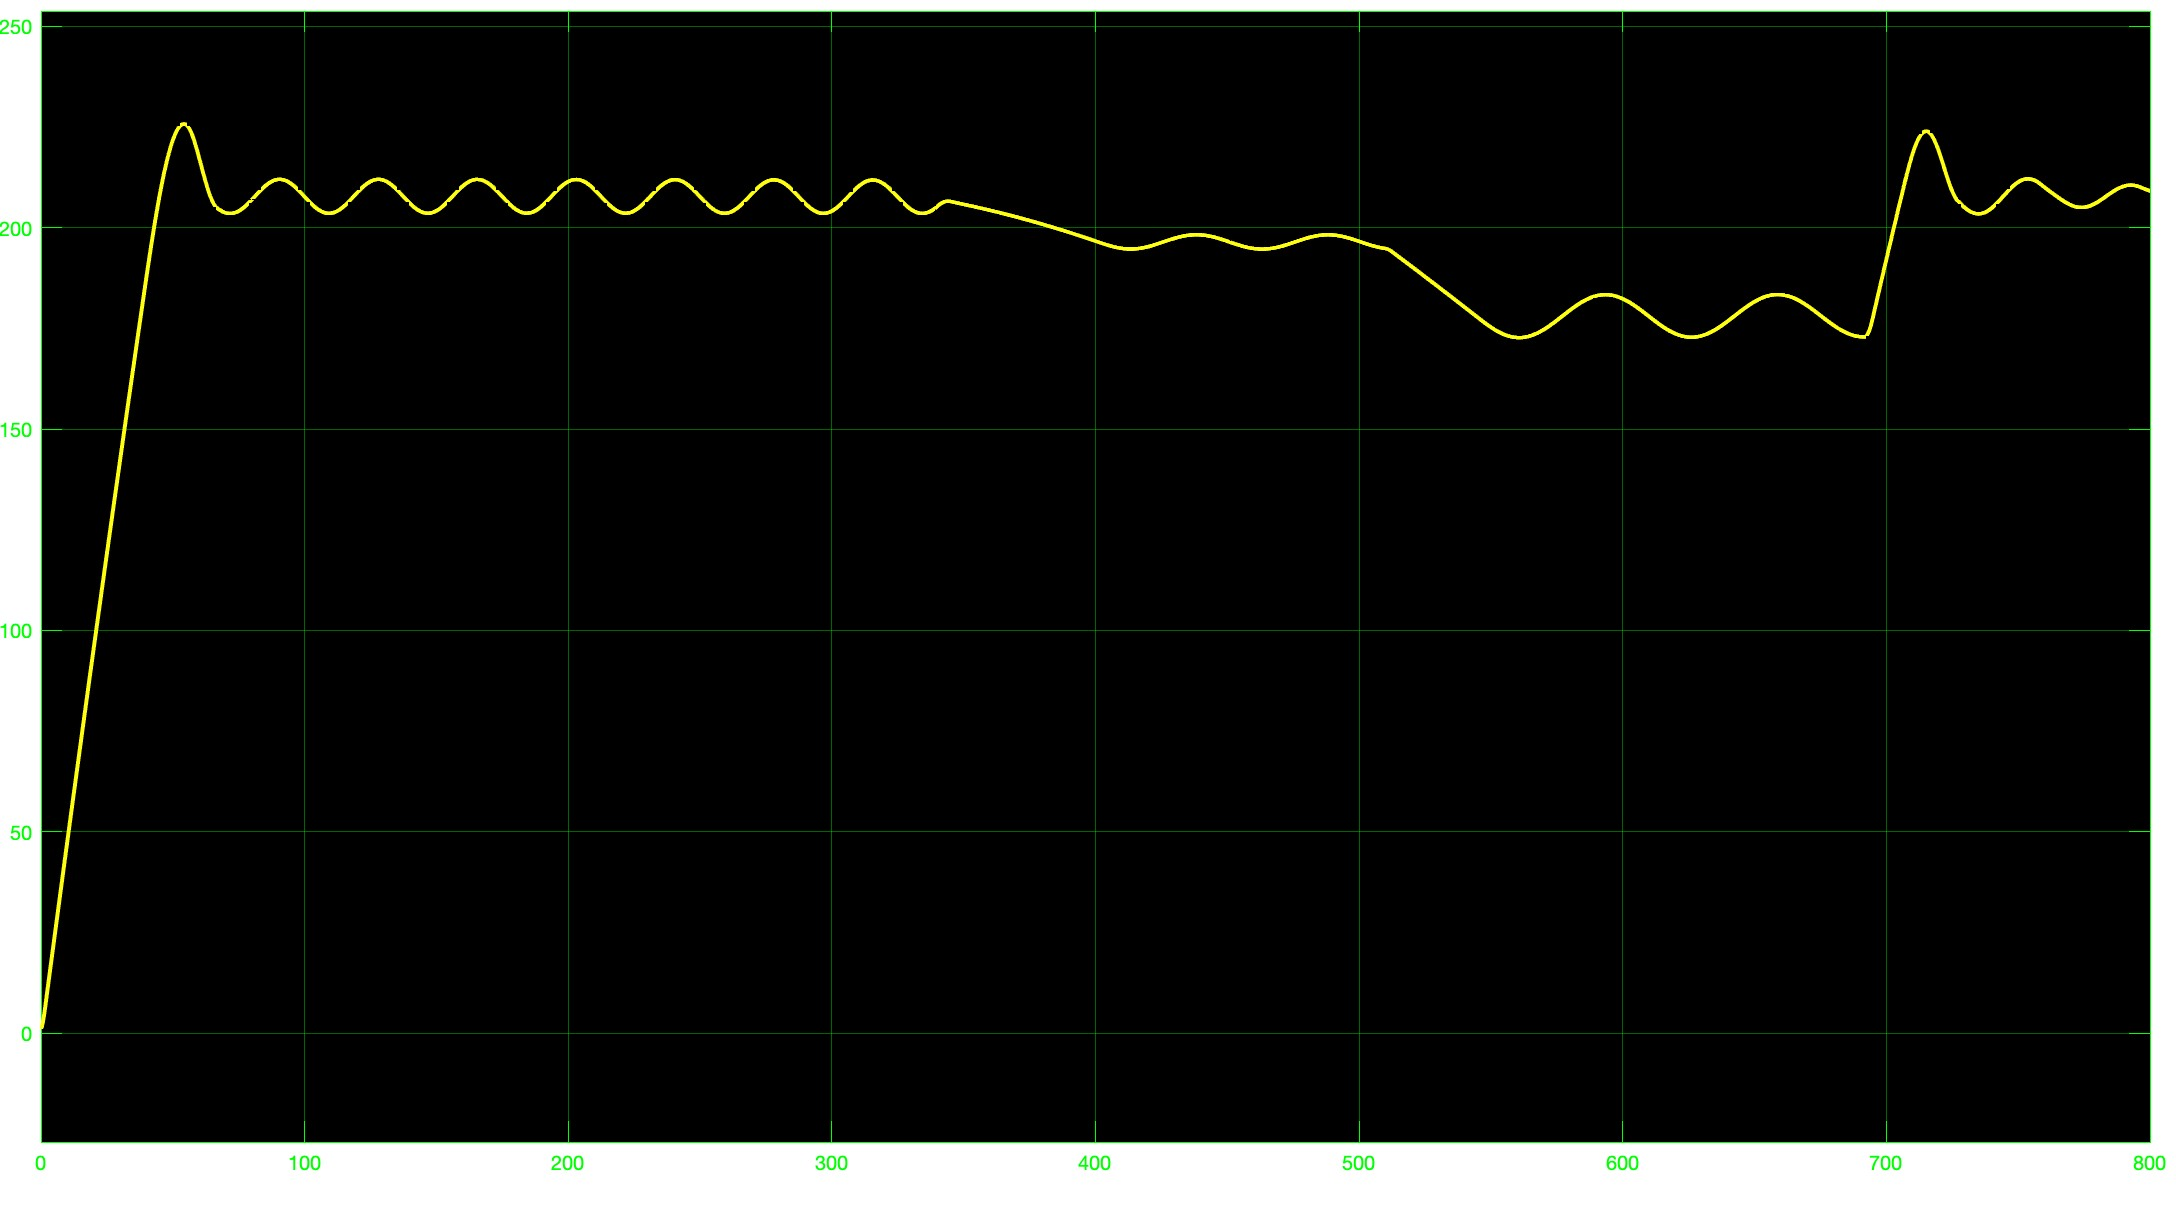
\includegraphics[scale=0.2]{Step_nonLineare/Step5_noLin.jpg}
    \caption{Risposta al gradino di ampiezza 5}
    \label{fig:enter-label}
\end{figure}

\begin{figure}[!h]
    \centering
    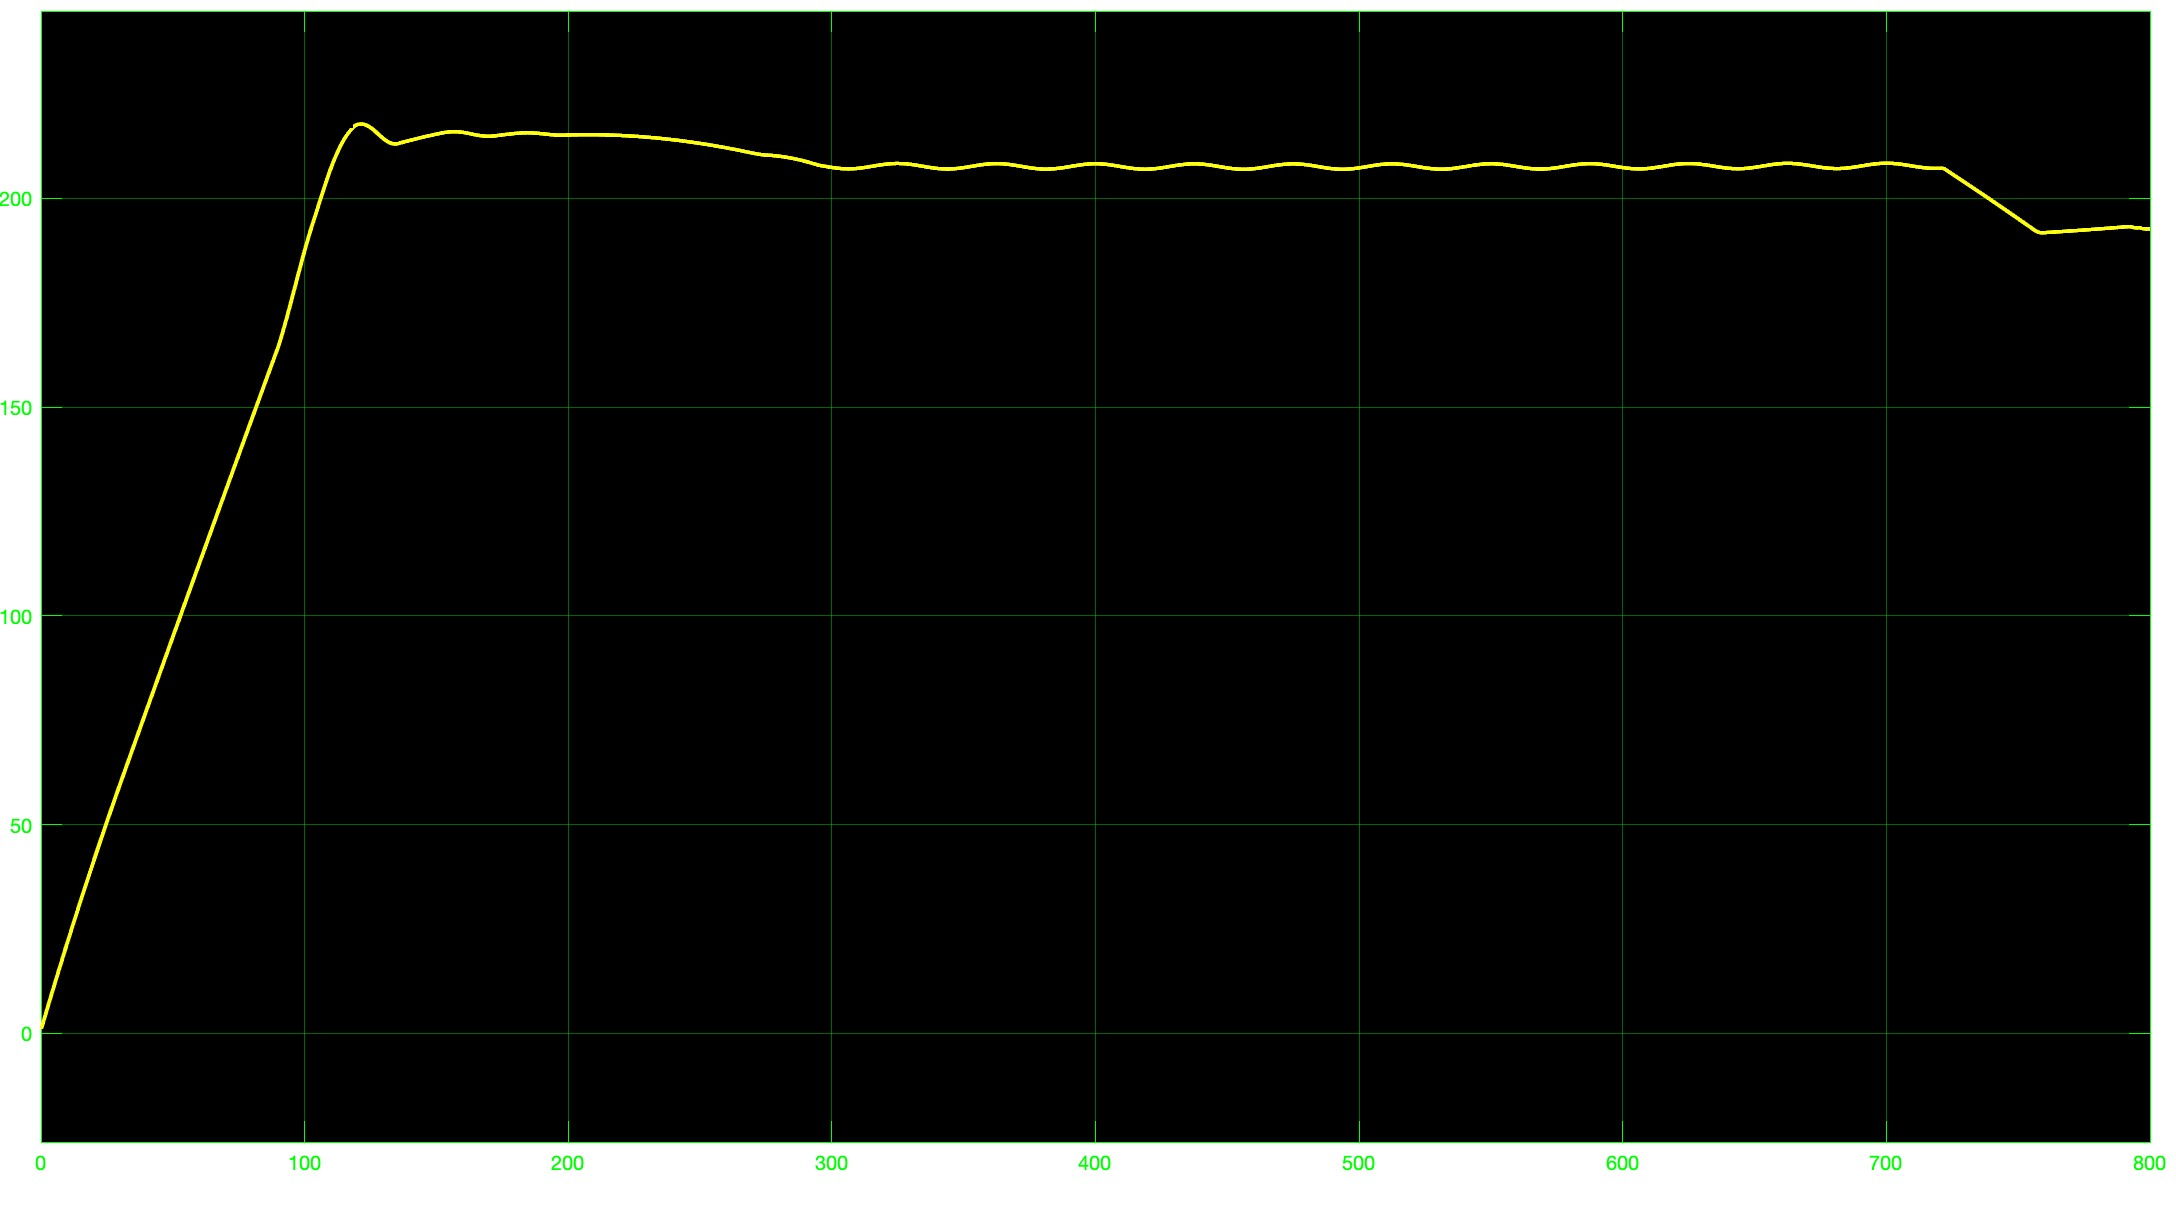
\includegraphics[scale=0.2]{Step_nonLineare/Step10_noLin.jpg}
    \caption{Risposta al gradino di ampiezza 10}
    \label{fig:enter-label}
\end{figure}


Per valori superiori a 5, dopo un certo intervallo di tempo, il sistema si allontana dalla stabilità, come evidenziato nelle Figure 27 e 28.

\clearpage

\section{Conclusioni}

Durante lo svolgimento del progetto, partendo dalla dinamica assegnata, fortemente non lineare, abbiamo provveduto alla linearizzazione del sistema, calcolo della funzione di trasferimento, progetto del regolatore per soddisfare le specifiche fornite e test del sistema linearizzato e non linearizzato. 

\vspace{0.3 cm}
I test sul linearizzato hanno rispettato tutte le specifiche fornite dal progetto, in termini di tempo di assestamento, non violazione dei vincoli su fase, disturbi e pulsazione minima e anche durante i test con disturbi di misura o disturbi sull'uscita non ci sono state discrepanze tra la risposta attesa e quella ottenuta.

\vspace{0.3 cm}
Discorso diverso per il sistema non linearizzato, la cui problematica più evidente ha riguardato il tempo di assestamento: seppure a fronte di variazioni sulle condizioni  iniziali il sistema ottenesse una risposta stabile, quest'ultima necessitava di un tempo di assestamento dell'ordine di $10^2$, valore che eccede di 3 ordini di grandezza quello imposto da specifica. Nella realtà, un sistema con una dinamica fortemente instabile come quello da noi analizzato non sarebbe proponibile a causa di un tempo di assestamento eccessivamente oltre le specifiche richieste. 
\end{document}
